\DocumentMetadata{}
\documentclass[manuscript,review,dvipsnames]{acmart}

\newcommand{\papertitle}{Too Many Issues: Automatically Prioritizing Analyzer Findings by Tracing Security Importance}
%Too Many Issues: Automatically Prioritizing Security Issues by Tracing Importance for the Project

\usepackage[utf8]{inputenc}
\usepackage{algorithmic}
\usepackage{graphicx}
\usepackage{textcomp}
\usepackage{xcolor}
\usepackage{caption}
\usepackage{refstyle}
\usepackage{listings}
\lstset{numbers=left,
numberstyle=\tiny,
numbersep=5pt,
xleftmargin=10pt%\parindent
}
\usepackage{float}
\usepackage{color}
\usepackage{enumitem}
\usepackage{tabularx}
\usepackage{subcaption}
\usepackage[linesnumbered,ruled]{algorithm2e}
%\usepackage[hyphens]{url}
\usepackage{booktabs}
%\usepackage[textsize=footnotesize]{todonotes}
\usepackage{footmisc} % For footnote references (in the list of authors)
\usepackage{balance}
\usepackage{csquotes}


\renewcommand{\algorithmautorefname}{Algorithm}
\renewcommand{\sectionautorefname}{Sec.}
\renewcommand{\subsectionautorefname}{Sec.}
\renewcommand{\figureautorefname}{Fig.}

\definecolor{red}{rgb}{1,0,0}
\newcommand{\appr}{\emph{Trace\-SEC}}

\usepackage{subcaption}

\usepackage{ifthen}
\usepackage{xparse}
\usepackage{calculator}
\usepackage{colortbl}
\newcommand\rcolor[1]{
    \ifthenelse{\lengthtest{#1pt < -10pt} }{\cellcolor{Red}#1\%}{
    \ifthenelse{\lengthtest{#1pt < -8pt} }{\cellcolor{Red!75}#1\%}{
    \ifthenelse{\lengthtest{#1pt < -6pt} }{\cellcolor{BurntOrange!75}#1\%}{
    \ifthenelse{\lengthtest{#1pt < -4pt} }{\cellcolor{YellowOrange!75}#1\%}{
    \ifthenelse{\lengthtest{#1pt < -2pt} }{\cellcolor{Goldenrod!85}#1\%}{
    \ifthenelse{\lengthtest{#1pt < -1pt} }{\cellcolor{Yellow!85}#1\%}{
    \ifthenelse{\lengthtest{#1pt < 1pt} }{\cellcolor{Yellow!40}#1\%}{
    \ifthenelse{\lengthtest{#1pt < 2pt} }{\cellcolor{ForestGreen!17}#1\%}{
    \ifthenelse{\lengthtest{#1pt < 4pt} }{\cellcolor{ForestGreen!33}#1\%}{
    \ifthenelse{\lengthtest{#1pt < 6pt} }{\cellcolor{ForestGreen!50}#1\%}{
    \ifthenelse{\lengthtest{#1pt < 8pt} }{\cellcolor{ForestGreen!67}#1\%}{
    \ifthenelse{\lengthtest{#1pt < 10pt} }{\cellcolor{ForestGreen!83}#1\%}{
    {\cellcolor{ForestGreen!100}#1\%}{\cellcolor{ForestGreen!100}#1\%}
    }}}}}}}}}}}}
}

%%
%% \BibTeX command to typeset BibTeX logo in the docs
\AtBeginDocument{%
  \providecommand\BibTeX{{%
    \normalfont B\kern-0.5em{\scshape i\kern-0.25em b}\kern-0.8em\TeX}}}

%\newcommand{\edit}[1]{\textcolor{blue}{{#1}}}
\newcommand{\edit}[1]{#1}

\acmJournal{TOSEM}
%\setcopyright{acmcopyright}
%\copyrightyear{2018}
%\acmYear{2018}
%\acmDOI{XXXXXXX.XXXXXXX}
%\acmPrice{15.00}
%\acmISBN{978-1-4503-XXXX-X/18/06}


\begin{document}

\title[\papertitle]{\papertitle}

\author[S. Peldszus]{Sven Peldszus}
\orcid{0000-0002-2604-0487}
\affiliation{%
  \institution{Ruhr University Bochum}
  \city{Bochum}
  \country{Germany}
}
\email{sven.peldszus@rub.de}

\author[K. Großer]{Katharina Großer}
\orcid{0000-0003-4532-0270}
\affiliation{%
  \institution{University of Koblenz}
  \city{Koblenz}
  \country{Germany}
}
\email{grosser@uni-koblenz.de}

\author[M. Konersmann]{Marco Konersmann}
\orcid{0003-3452-57722}
\affiliation{%
 \institution{ista SE}
 \city{Essen}
 \country{Germany}
}

\author[W. Brunotte]{Wasja Brunotte}
\orcid{0000-0003-4127-6508}
%\affiliation{%
%  \institution{Leibniz University Hannover}
%  \city{Hannover}
%  \country{Germany}
%}


\author[M. Ahrens]{Maike Ahrens}
\orcid{0000-0002-9577-0598}
%\email{maike.ahrens@inf.uni-hannover.de}

\author[K. Schneider]{Kurt Schneider}
\orcid{0000-0002-7456-8323}
\email{kurt.schneider@inf.uni-hannover.de}
\affiliation{%
  \institution{Leibniz University Hannover}
  \city{Hannover}
  \country{Germany}
}

\author[J. Jürjens]{Jan Jürjens}
\orcid{0000-0002-8938-0470}
\affiliation{%
  \institution{University of Koblenz}
  \city{Koblenz}
  \country{Germany}
}
\additionalaffiliation{%
  \institution{Fraunhofer Institute for Software and Systems Engineering (ISST)}
  \city{Dortmund}
  \country{Germany}
}
\email{juerjens@uni-koblenz.de}

%\renewcommand[1]{\shortauthors}{Sven Peldszus, Katharina Großer, Marco Konersmann, Wasja Brunotte, et al.}

%
\begin{abstract}
Code-based analyzers often find too many potentially security-related issues to address them all. Therefore, issues likely to lead to vulnerabilities should be fixed first. Such prioritization requires project-specific knowledge, such as quality requirements, security-related decisions, and design, not accessible to code analyzers. We present TraceSEC, an automated technique for prioritizing issues according to their security-related importance to the project. Its key concept is to include available design artifacts and trace links between them, thus capturing the project context code lacks. We reduce the problem of issue prioritization to a maximum flow problem and quantify the importance of each issue by the flow from user-defined quality aspects to it, i.e., quantifying its impact on project-specific security preferences. Our evaluation shows that TraceSEC effectively provides automated prioritization and can be tailored to project-specific quality goals. Its prioritization correlates stronger with manual expert prioritization than SonarQube rule severities, commonly used in practice. In particular, TraceSEC has a higher similarity for identifying high-priority issues. Even projects with only imperfect traceability or planning artifacts benefit from TraceSEC, it scales reasonably well for codebases up to 4~million lines of code, and the initial setup overhead is likely to be recouped after the first automated prioritization
%
%Static code analysis plays an essential role in the quality assurance of software systems, especially concerning security. However, code-based static analyzers often detect too many potential security issues to resolve them all with reasonable effort. Therefore, issues that are likely to lead to vulnerabilities should be fixed first. Such prioritization requires a lot of information about the project, such as quality requirements, security-related decisions, and design. Code-based static analyzers do not have this information and therefore cannot properly assess the importance of issues. Also, the prioritization of detection rules cannot fully reflect the importance as perceived by developers. We present TraceSEC, an automated approach to prioritizing issues in a codebase according to their security-related importance to the project. The key concept is to include in the prioritization artifacts that are created manually during development anyway, thus capturing the project context that is not available in the source code, and the trace links between them. Prioritization starts from a quality model in which experts and stakeholders determine the relative importance of quality aspects, e.g. related to security, and follows trace links across different artifacts, such as requirements and design models, to the issue locations in the source code. We reduce the problem of trace-based issue prioritization to a maximum flow problem and quantify the importance of each issue by the flow of user-defined quality aspects to it. Our evaluation shows that TraceSEC effectively provides automated prioritization and can be tailored to project-specific quality goals. The prioritization has a stronger Spearman rank correlation at a significance level of 0.01 with a manual expert prioritization than one based on the SonarQube rule severities, and in particular, has a higher similarity for identifying high-priority issues. We show that our technique scales reasonably well for codebases of up to 4~million lines of code on a developer notebook.
\end{abstract}

%CCS Concepts https://dl.acm.org/ccs#
\begin{CCSXML}
<ccs2012>
   <concept>
       <concept_id>10011007.10011006</concept_id>
       <concept_desc>Software and its engineering~Software notations and tools</concept_desc>
       <concept_significance>500</concept_significance>
       </concept>
   <concept>
       <concept_id>10002978.10002986</concept_id>
       <concept_desc>Security and privacy~Formal methods and theory of security</concept_desc>
       <concept_significance>500</concept_significance>
       </concept>
   <concept>
       <concept_id>10002978.10003006</concept_id>
       <concept_desc>Security and privacy~Systems security</concept_desc>
       <concept_significance>500</concept_significance>
       </concept>
   <concept>
       <concept_id>10011007.10011074</concept_id>
       <concept_desc>Software and its engineering~Software creation and management</concept_desc>
       <concept_significance>300</concept_significance>
       </concept>
 </ccs2012>
\end{CCSXML}

\ccsdesc[500]{Software and its engineering~Software notations and tools}
\ccsdesc[500]{Security and privacy~Formal methods and theory of security}
\ccsdesc[500]{Security and privacy~Systems security}
\ccsdesc[300]{Software and its engineering~Software creation and management}

%%
%% Keywords. The author(s) should pick words that accurately describe
%% the work being presented. Separate the keywords with commas.
\keywords{static code analysis, security issues, traceability, issue prioritization}

%\begin{IEEEkeywords}
%static code analysis, security issues, traceability, issue prioritization
%\end{IEEEkeywords}


\maketitle

%\newpage
\section{Introduction}
\label{sec:intro}
\noindent
While considering security as a core aspect early in the development of software-intensive systems is becoming increasingly important and adopted in practice\,\cite{10.1145/3468264.3473926,Peldszus2025}, vulnerabilities still reside in the concrete implementation of a system.
Nevertheless, planning for security, i.e., designing a secure architecture\,\cite{1281254}, taking into account typical threats and best practices that have proven to be secure, is one of the most important steps in the development of a secure software.
The planned security design builds the foundation for the actual system and must be implemented in code\,\cite{1281254,10.1145/3385678.3385687}.
However, because it is a common misconception that developers are well informed about software security\,\cite{Ryan2023}, it is likely that developers will make security-related mistakes. As a result, implementations often contain vulnerabilities that are either immediately exploitable or that invalidate assumptions made in the security design, such as exposing data considered critical in the design to other spheres of influence.%
\edit{
    Unfortunately, such security-critical mistakes are often hidden by many other flaws concerning qualities such as maintainability.
    Furthermore, since the primary incentive of developers is to provide functionality, even though they consider security to be important, they prioritize functionality over security\,\cite{Peldszus2025}, and therefore may tend to fix problems that complicate the implementation of functionality instead of searching for security issues and fixing them.
}

To help in identifying and fixing potential security-related mistakes, state-of-the-art static analyzers like \emph{SonarQube}\,\cite{sonar}, which is widely deployed in many development pipelines, focus on detecting code smells, or bugs and flaws that resemble them.
Code smells are locally confined anomalies that can be detected without a thorough examination of the context\,\cite{peldszus2016continuous}. They are usually at the level of classes, methods, or individual code statements.
This local restriction allows for easy automated detection with high accuracy.
%\cite{Walden2014} low precision for vulnerabilities
Unfortunately, static analysis tools show overwhelmingly many issues---too many to address when applied to typical, non-trivial codebases.
The vast number hardly helps developers to increase security\,\cite{Walden2014}.
E.g., the \emph{iTrust Electronics Health Records} system\,\cite{heckman2018}, a web application for managing patient data and procedures with 77,501~logical lines of code,
%developed as a class project %at the North Carolina State University %over 25 semesters
%\cite{heckman2018},
already has 6,284 issue findings in SonarQube (1,352 in productive and 4,932 in test code).
%Throughout this paper we are going to use the \emph{iTrust Elecronics Health Records} system as running example. The iTrust system is a web application for managing patient data and procedures. The system has been developed as a class project at the North Carolina State University over 25 semesters \cite{heckman2018}. The iTrust system has been implemented using Java and Java Server Pages~(JSP).
%
%What is more,
%Following up on all of those warnings is infeasible as it would require enormous resources.
Not every unfixed code smell is sufficient to open an exploitable attack vector\,\cite{Walden2014}, but some may predict vulnerabilites\,\cite{8819456,9359268}, and classes with issues are generally more error-prone\,\cite{FV15}.
%For a successful attack, a combination of multiple essential unfixed code smells at a sensitive location of the system is necessary.
%Few essential unfixed code smells
Combinations of smells, or those at sensitive locations, can have a severe impact.
%Due to the overwhelming number of issues%less crucial warnings
%However,
Yet,
due to overwhelmingly many issues, developers are overstrained and often overlook the few essential ones, i.e, %they misjudge
misjudging
their importance in respect to the design of the system.
Lack of resources for fixing all issues is a major reason for releasing code with known vulnerabilities:
48\% of the participants in a survey of the Enterprise Strategy Group frequently release code with known security issues\,\cite{Gruber2020}.

Since complete security is not feasible\,\cite{Mazurek2022}, i.e., not having the resources to fix all identified issues, a prioritization of the usually vast number of identified issues is required to fix the ones with the highest impact first\,\cite{Walden2014}, i.e., those that lead to violating assumptions of the planned security design. To this end, tool-assisted prioritization of issues in order to solve the most important issues first helps to reduce the severity of releasing software, even with limited resources.
Recent research mostly focused on identifying detection rules that are more critical than others\,\cite{FV15}, still leaving developers with dozens of critical rules and still hundreds or thousands of issues, or prioritizing issues in a way that as many as possible can be fixed with as few effort as possible without considering their precise impact on the project\,\cite{AB19}.
However, it has been shown that the severity of rules, e.g., in SonarQube, is misleading\,\cite{Katin2022} and that there is a lack of, but need for, approaches that consider the development context\,\cite{Pina21}.
Often, static analyzers cannot prioritize issues effectively because they lack information about the project context that determines the importance of a warning\,\cite{Walden2014}, which is mostly %determined
shaped
by requirements and design.
Incorporating this information helps, %for example,
e.g.,
by proposing to fix issues in security-critical parts of the system first.
Prioritization is usually performed manually, e.g., by developers when deciding which issues to fix.
Thereby, they must perform a risk assessment to evaluate the issues concerning their likelihood and possible impact, taking into account, besides technical details, project-specific knowledge\,\cite{shedden2011incorporating}.
Since it is usually not feasible to systematically consider all available information manually, and it is not scalable, this manual approach does not ensure that the most urgent and important issues are fixed first.

\begin{samepage}
Our \emph{goal} is to automatically prioritize issues reported by code-based static analyzers.
We do not aim to increase the accuracy of these analyzers by reducing false positives
or to filter results, but rather to sort their output by security importance as it is.
We consider the following \emph{research~question}:

%\newline
%\vspace{.1pt}%
%\smallskip
\begingroup
\leftskip=0cm plus 0.5fil \rightskip=0cm plus -0.5fil
\parfillskip=0cm plus 1fil
\noindent
\emph{\enquote{How can project context information be systematically used to prioritize %security
issues reported by code analyzers according to
their relevance for the security of the project?}}%
\par
\endgroup
%\vspace{.1pt}%
%\smallskip
\end{samepage}

\noindent
Relevance in this context is defined as the strength of an issue's connection to the project-specific security qualities captured in a quality model, i.e., how many of them can be affected by a specific issue and how directly.
In many projects, standards such as the ISO/IEC 62304 for medical device software\,\cite{IEC62304}, require creating detailed planning artifacts and trace links between the development artifacts\,\cite{tracing}: code is based on design, which is based on requirements, and many other relations can be captured\,\cite{schwarz2010gbt,ISO24765:2010,spanoudakis2005software}.

In this paper, we propose to reuse those trace links to decide which issues to solve first.
We map the prioritization based on those trace links to an maximum flow problem\,\cite{harris1955}, a graph theoretical problem to which many connectivity-based optimizations are mapped.
In our case, this problem is used to quantify the connection between issues and project-specific security qualities, i.e., the relevance of an issue.
In general, our technique \appr{} supports arbitrary artifacts among which trace links exist and that can be represented as models.
For practicality reasons, we consider in our evaluation requirements, architecture models, and program code, and propose to use a quality model\,\cite{Deissenboek2009,Schneider2012ASQ,WAGNER2015101} as core reference in security planning and prioritization.
\appr{} comprises three steps as shown in \autoref{fig:PrioApproach}:



\begin{figure}
	\centering
	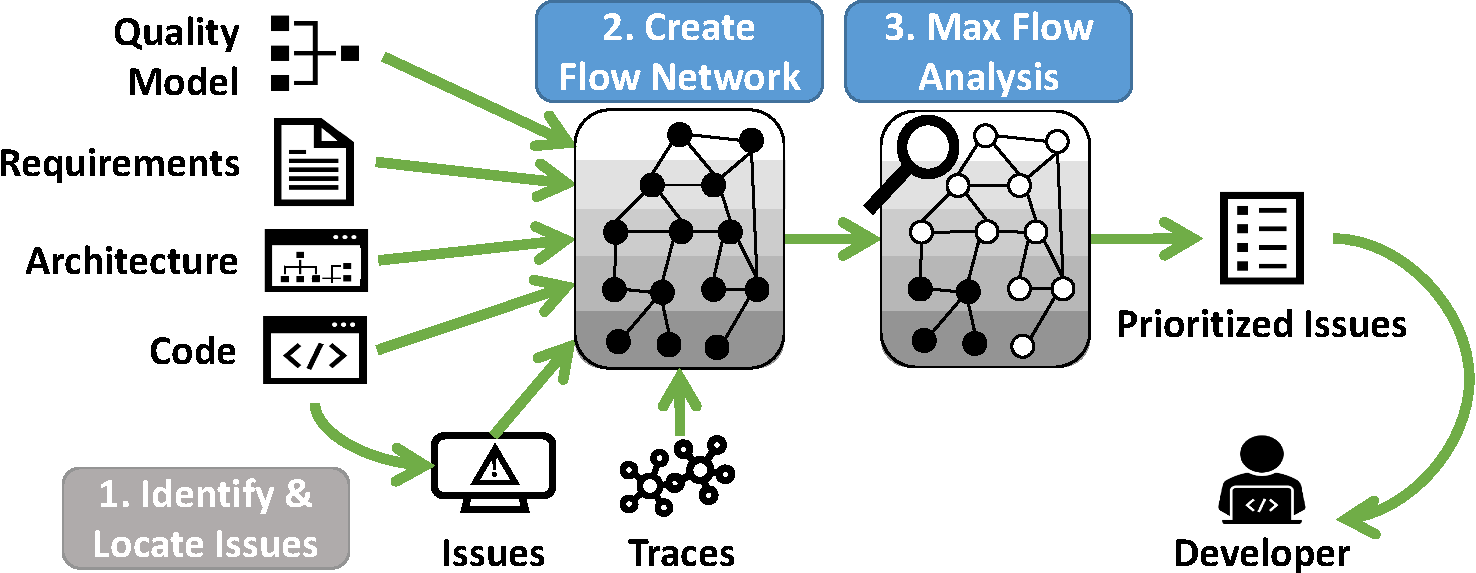
\includegraphics[width=.6\columnwidth]{figures/Gesamtschaubild-v05-KG.pdf}%width=0.8\textwidth
	\caption{Concept of the Issue Prioritization Technique}
	\label{fig:PrioApproach}
\end{figure}

\begin{enumerate}[label=\arabic*.]
    \item First, we \emph{identify and locate %security
    issues} with current static analysis tools. %, e.g., SonarQube.
%We do not propose new static analysis methods in this work but rely on state-of-the-art technology that is widely used in practice.
%%This usually results in a large list of issues.
%%It is unclear which of these issues should be addressed first as it is not clear which ones are actually security-relevant because they are located in a critical part of the implementation and can be exploited.
%Our main contributions reside in %the following
%steps 2 \& 3 (highlighted in \autoref{fig:PrioApproach}).

\item Second, we \emph{create a flow network of trace links} between the available development artifacts and these issues, thus embedding contextual knowledge into the prioritization.
To reflect the importance of different trace links, we apply capacities to them %the trace links
based on the linked artifact types and their interrelations.

%A quality model\,\cite{Deissenboek2009,Schneider2012ASQ,WAGNER2015101} is used to organize the quality goals and detail them to quality requirements. It serves as a core %element
%reference
%in security planning and prioritization and enables us to prioritize security issues in a later stage. However, our approach supports arbitrary artifacts that can be mapped to models and among which trace links exist.

\item Third, we \emph{analyze the flow network of interconnected artifacts} to calculate the security-related priorities of issues by reducing the prioritization to the \textit{maximum flow problem}\,\cite{harris1955} for each identified issue.
With this algorithm, we calculate a priority for each issue instance found by a static analysis tool, by following the trace links.
This priority reflects the connection between the issue and the project's security preferences captured in qualities, indicating the potential impact on the preferred security qualities.
\end{enumerate}

\noindent
If a static code analysis tool detects %security
issues, using \appr{}, the developer can focus on the most important issues first.
%
We do not propose new static analysis methods in this work but rely on state-of-the-art technology that is widely used in practice.
%This usually results in a large list of issues.
%It is unclear which of these issues should be addressed first as it is not clear which ones are actually security-relevant because they are located in a critical part of the implementation and can be exploited.
Our main contributions reside in %the following
steps 2 \& 3 (highlighted in \autoref{fig:PrioApproach}).
%
To this end, the contributions presented in this paper are:

\begin{itemize}
    \item The \appr{} issue prioritization technique that leverages project-specific knowledge captured in project artifacts as well as trace links and maps the issue prioritization itself to a maximum flow problem.

    %\item A domain-specific language (DSL)\,\cite{fowler2010domain,dsl} that allows arbitrary model-based artifacts to be supported in prioritization, and to tailor the prioritization based on how different artifacts are used in individual projects.

    \item Publicly available open source tool support, which comes with a domain-specific language (DSL) that allows arbitrary model-based artifacts to be supported in prioritization, and to tailor the prioritization based on how different artifacts are used in individual projects. We provide specifications written in this DSL\,\cite{fowler2010domain,dsl}
    for supporting UML models\,\cite{uml}, a program model for Java programs\,\cite{peldszus2016continuous,Peldszus2022}, as well as our own publicly available metamodels for quality models and requirements\,\cite{replication}.

    \item An evaluation of \appr{} concerning
    \begin{itemize}
        \item its effectiveness in issue prioritization in comparison to widely used state-of-the-art rule priorities,
        \item how well project specific security requirements can be considered in the prioritization based on preferences specified in quality models,
        \item the scalability of \appr{} in the context of large projects and the involved overhead for using it, and
        \item the impact of imperfect trace links and planning artifacts on the prioritization.
    \end{itemize}

    Evaluation results show that our prioritization is closer to manual prioritization than prioritization based on SonarQube rule priorities, that project-specific preferences captured in a quality model indeed influence the issue prioritization, and that our technique scales well even for large software projects.
\end{itemize}

\noindent
	We provide practitioners and tool builders with insights on how to automatically include planning artifacts into the prioritization of issues detected by static analyzers.
	We provide researchers with first insights of how traceability affects prioritization and the means to investigate the relationship between implementation-level issues and security planning artifacts, i.e., the security design, in depth.

This work is structured as follows.
First, we give the required background in \autoref{sec:background} and introduce our prioritization technique in detail in \autoref{sec:approach}.
To this end, we first discuss different artifacts commonly created during systems development and the relations among them that could be leveraged by \appr{} in \autoref{DevArt}.
Based on these artifacts, we introduce how to extract a flow network from them in \autoref{sec:flownetwork}. We discuss how to systematically tailor the flow network construction towards potentially varying needs due to project context or the used artifacts and introduce a domain-specific language~(DSL) that allows the reusable specification of such tailoring in \autoref{sec:dsl}.
In \autoref{sec:tool} we introduce the tool support of \appr{} that is leveraged for the evaluation of \appr{}, which is presented in detail in \autoref{sec:eval}.
We close the work with a discussion in \autoref{sec:disc},
%where we consider assumptions and implications in \autoref{sec:implication} and threats to validity in \autoref{sec:threats},
related work in \autoref{sec:rw}, and a conclusion in \autoref{sec:conslusion}.
\section{Background}
\label{sec:background}
%In this section,
This section gives a short overview of security engineering, trace links, and maximum flow analysis as used in \appr.

\edit{
\subsection{Vulnerabilities and Weaknesses}
A vulnerability is a flaw in a software system that an attacker can exploit to compromise its confidentiality, integrity, or availability\,\cite{Shahriar2012,NVD2021, OWASP-Top10}.
Examples include security-critical bugs in the source code and missing security features that leave the system susceptible to attacks.
Vulnerabilities often stem from underlying issues in the software's design, implementation, or configuration.
Exploitation of these vulnerabilities can lead to severe consequences, such as data breaches, unauthorized access, or service disruption\,\cite{Telang2007}.
%
The faults behind vulnerabilities are generally categorized into broader conceptual weaknesses, which represent classes of vulnerabilities sharing similar root causes\,\cite{cwe}.
For example, weaknesses such as buffer overflows, input validation errors, and insecure authentication mechanisms fall under these categories
Consequently, a specific vulnerability is an instance of one or more of these weaknesses.
%
In software analysis, static code analyzers often detect vulnerabilities by examining source code for security issues \cite{Shahriar2012}.
These tools are usually designed to identify specific code patterns or constructs that reflect specific weaknesses, thereby detecting potential vulnerabilities.
}

\subsection{Security Engineering Practices}
Best practices in security engineering are critical to ensuring the development of secure and robust software systems\,\cite{1281254}.
By integrating security into every phase of the software development process, organizations can proactively identify and address vulnerabilities, protect sensitive data, and minimize the risk of security breaches\,\cite{9669954}.
In the process, various security-related artifacts are created, such as starting with abstract security goals that are refined into project-specific security requirements\,\cite{turpe2017trouble}, and later to a secure architecture\,\cite{4359475}.
In practice, artifacts often stem from less integrated processes but are still created frequently, such as documenting the results of a risk assessment\,\cite{SHAMELISENDI201614,BRUNNER2020101776}.

Many security-related standards for the development of critical software systems, such as ISO/IEC\,62304\,\cite{IEC62304}, require such a systematic analysis of potential threats and vulnerabilities early in the development process.
Identifying assets, potential attackers, and attack vectors is essential for prioritizing security requirements and designing appropriate countermeasures\,\cite{TUMA2018275}.
Security certification standards such as the \emph{Common Criteria}\,\cite{cc} provide a framework to support this process and require explicit documentation of these practices, including the artifacts produced. Such artifacts include, but are not limited to, architecture documentation and related security considerations, planned countermeasures, and documentation of risk assessments, including identified risks and their impact, if they occur.
Developers then implement the planned functionality, security requirements, and countermeasures.

While such security standards and the artifacts that must be delivered are often oriented on traditional development processes such as the V model\,\cite{MuellerEttrich1997}, they usually do not require to follow a specific development process.
Standards define security-related engineering steps that must be performed and documented, i.e., system design and risk assessment documented in the form of a system architecture and corresponding documents capturing threats, likelihoods, and possible impacts in relation to this architecture.
Still, there is often a perceived conflict with today's trending agile development processes.
Particularly model-based system development is often seen as conflicting with agile development processes, although the feasibility of agile model-based development processes has explicitly been shown\,\cite{Gray2018}.

At the implementation level, secure coding practices, such as the CERT Oracle Secure Coding Standard for Java\,\cite{long2011cert}, can help minimize the introduction of vulnerabilities.
Guidelines and security principles such as those provided by OWASP\,\cite{secure-coding}, which include principles such as input validation, output encryption, and proper error handling, also help to implement secure software systems.
In addition, tools can statically check for compliance with best practices\,\cite{sonar} as well as many violations of security principles.
Overall, tool support, particularly in the form of static security analyzers\,\cite{BCP+13}, is essential to an effective security engineering process.
However, as discussed earlier, the output of such tools is likely to be overwhelmingly large\,\cite{Walden2014}.

Many security engineering approaches explicitly combine several artifacts to support security engineering, such as requirements, UML models annotated with the UMLsec\,\cite{jurjens2005secure} security profile, and security standards such as the Common Criteria\,\cite{houmb2010eliciting}, other combine
SecBPMN models\,\cite{Salnitri2017DSB} and security oriented goal models\,\cite{Salnitri2020},
risk models and requirements\,\cite{5507389}, or design models and source code\,\cite{Peldszus2022}.
Tracing, for example of security requirements, is typically a key component of these approaches and is also essential for security maintenance\,\cite{Yu2008}.
For this reason, security standards such as the Common Criteria\,\cite{cc} not only ask for artifacts documenting the security considerations but also require traceability for security-related decisions.


\subsection{Trace Links \& Trace Link Management}
\label{sec:background:tracelinks}
%\subsubsection{Trace Links and Traceability}
In software engineering, trace links (%also referred to as
or
traceability links)  are explicit interrelations between multiple development artifacts (e.g.,\,\cite{schwarz2010gbt}).
Those links have to be distinguished from traces, which are recorded software execution paths\,\cite{Praehofer2014,Hendriks2016}. ISO/IEC/IEEE\,24765\,\cite{ISO24765:2010} describes traceability as \enquote{the degree to which a relationship can be established between two or more products of the development process, especially products having a predecessor-successor or master-subordinate relationship %to one another
[\dots]}. There are mainly two communities using trace links\,\cite{winkler2010survey}: %The r
Requirements engineering %community
uses %trace links
them
to trace requirements to design and implementation and back\,\cite{Gotel1994Trace,Pinheiro2004trace}, while model-driven software engineering uses trace links among design artifacts (e.g.,\,\cite{Mouratidis2010GDS,Ahmadian2017MBP}) or models and code~(e.g.,\,\cite{Peldszus2019SDF}).

Possibilities to establish trace links range from simple references of complete documents to individual, identifiable, typed, and possibly attributed connections between particular elements within development artifacts. %Winkler and von Pilgrim\,\cite{winkler2010survey} surveyed approaches for specifying and maintaining trace links in requirements engineering and model-driven development.
Different approaches exist to specify and maintain \cite{winkler2010survey} various types of trace links %exist
\cite{spanoudakis2005software,Espinoza2006ASC}.
We aim at explicit, material, and typed links conforming to a traceability model \cite{Pinheiro2004trace,schwarz2010gbt,Grosser2022RDR} defining the possible trace links and traceable objects.

%\subsubsection{Tool Support for Trace Link Management}
Various works support establishing and maintaining trace links between a system's implementation and its design models.
E.g., %the
\emph{GRaViTY}% framework
\,\cite{PKLS2015,PBKJ2021,Peldszus2022} %utilizes
uses
\emph{triple graph grammars}~(TGG)\,\cite{schurr1994specification} to synchronize changes between the implementation and design-time UML models.
Thereby, a correspondence model is built that contains all trace links.
Similarly, the \emph{Codeling} tool \cite{Konersmann2018OEM, Konersmann2018EIA} relates models with code by developing mappings between design model elements and recurring code structures.
Correspondences are defined on the type level, rather than the instance level.
To this end, a model can be extracted from the source code, and changes in a model can be propagated to code.
Trace links solely within or between artifacts of the same type are also exploited.
E.g., the \emph{T-Reqs} framework\,\cite{Grosser2022RDR} uses trace links
%managed in a \emph{Neo4J} graph
to identify completeness and consistency flaws in requirements over different abstraction levels to support the integration of reusable requirements.
In \emph{single underlying model} (SUM\,\cite{Meier2020,Atkinson2010}) approaches, all artifacts, including requirements, design models, but also code models, should be maintained in a single model that provides trace links among them.

Besides maintaining trace links from the beginning of development, some approaches allow reconstructing trace links. % after the fact.
%For data flow diagrams~(DFDs), Peldszus et al.\,\cite{Peldszus2019SDF,TPS2022} propose a semi-automated approach for constructing trace links between the DFDs and their implementation. Such approaches exist for many artifact types \cite{Rasiman2022,Merten2016,Samer2019NAI,Wang2020DSS,Goknil2014}.
For data flow diagrams (DFDs), which are widely used for threat modeling, semi-automated approaches allow the construction of trace links between the DFDs and their implementation\,\cite{Peldszus2019SDF,TPS2022}.
Similar approaches exist for many other artifact types\,\cite{Rasiman2022,Merten2016}.
Among others, there is work on detecting dependencies between requirements\,\cite{Samer2019NAI,Wang2020DSS}, recovering trace links between requirements and the architecture\,\cite{Goknil2014,Keim2024},
between requirements and source code\,\cite{10.1145/2491627.2491633,Hey2024}, and between the architecture and source code\,\cite{keim2021trace}.
Other research goes into the direction of automatically completing incomplete sets of trace links, e.g., between entries in issue trackers and commits\,\cite{rath2018}.

\subsection{The Maximum Flow Problem}
\noindent
The maximum flow problem is a common problem in graph theory\,\cite{harris1955} to which we will reduce the problem of issue prioritization.%
This problem is commonly used to express connectivity in graphs\,\cite{Esfahanian2013}, such as how strong two nodes are connected.
In practice, this is applied for optimization problems such as flight crew planning, dimensioning telecommunication networks, or optimizing transportation\,\cite{Feng2012}.
We consider a project's security preferences captured in relevant security qualities to be the core reference for security planning and engineering.
Therefore, we want to prioritize issues according to the strength of their connection to those of these qualities they could affect, which can be seen as an instance of a maximum flow problem.

Given a flow network, that is, a directed graph $G = (N,E)$ consisting of nodes $n \in N$ and directed edges $e \in E$ with capacities~$w$, the question of the maximum flow problem is how large is the network capacity between a specific source and sink, i.e., the maximum flow.
This can be thought of as the number of flow tokens that can be propagated from a source, which acts as an infinite source of flow tokens, to a sink, which consumes all tokens that can reach it.
No more tokens can be sent over each edge than its capacity~$w$ indicates.
The higher the maximum flow between two nodes, the stronger the connection between those two nodes.

Various algorithms solve the maximum flow problem efficiently.
The best complexity is strongly polynomial.
Two major algorithms %for solving the problem
are Ford-Fulkerson's\,\cite{ford_fulkerson_1956} and Dinic's\,\cite{dinic1970algorithm} algorithms.
The former has a complexity of $\mathcal{O}(E|f_{max}|)$ where $f_{max}$ is the flow with maximum value.
Dinic's algorithm performs better with $\mathcal{O}(VE\log(V))$ when a dynamic tree data structure is used.
In \appr{}, we implement Dinic’s algorithm.
\section{Prioritizing Issues by Solving a Maximum Flow Problem}
\label{sec:approach}
%
In \appr, we apply the maximum flow problem to determine the security relevance of issues:
What is the maximum flow from the quality model to each issue, i.e., how strongly is the issue connected to the project's security preferences?
Thus, we reduce the prioritization problem to instances of the maximum flow problem.
The project-specific basis according to which issues will be prioritized is established in a human-based discussion process that leads to a quality model.
For example, the first step of Microsoft's Security Development Lifecycle consists of establishing security standards, metrics, and governance\,\cite{howard2006security}, which should be captured in a quality model.
In this process, priorities are assigned to quality aspects according to their importance for the project's security.
As part of the issue prioritization, those quality priorities are fully automated propagated over to subsequent artifacts that are derived from the quality aspects during regular system development, e.g., requirements or design models.
%We interpret this as a "flow" of relevance along the refinement and development activities. Traces of these activities ("A reads X, then writes Y" $\rightarrow$ trace from X to Y) are modeled as pipes.
In the end, relevance flows from the quality model along the trace links to the issues detected in the implementation, e.g., by SonarQube.

    The issues that analyzers can detect are often associated with the weaknesses of which they are an instance\edit{, e.g., the detection rules of SonarQube\,\cite{sonar} are often linked to relevant weaknesses in the Common Weakness Enumeration (CWE)\,\cite{cwe}}.
    Since different weaknesses can affect different security qualities captured in the quality model, this information helps developers assess the impact of an issue.
    However, it is only part of what they need to consider.
    Typically, developers also consider other aspects, such as where an issue is found in relation to the security design of the system, when assessing its impact.
	While issues detected by analyzers reside in the low-level implementation, e.g., buffer overflow vulnerabilities, and are usually absent from higher-level system models or requirements, these explicitly contain information about what is planned to be the most security-critical parts of the system, which is absent from the implementation.
	However, this information must be considered when prioritizing issues according to their potential security impact.
	Therefore, in addition to the quality model, detected issues, and how the weaknesses of which they are instances are related to the quality model, we also include available planning artifacts into the flow network that we use for calculating the maximum flow, i.e., prioritizing issues.
	Issues that accumulate more security relevance through direct, i.e., the relationship between weaknesses and security qualities, and indirect trace links, i.e., through design models used for security planning to security qualities, are stronger connected to security-critical parts of the system and its security qualities, are are therefore prioritized over others.

	In the prioritization, we also have to consider that different kinds of relationships can vary in their impact on the priority of an issues.
	For example, consider a security-critical module of the system.
	While all elements contained in this module are likely to be also security-critical and an issue within them could have a high impact on the security of the system, the immediate impact of an issue on other elements that are accessed from within this security-critical module is lower.
	We reflect this by automatically assigning capacities to the edges of the flow network according to the type of relation ship and trace link, thereby also lowering the impact of longer transitive propagation.

	    In \appr{}, we consider three aspects in the prioritization of issues concerning their security impact on the project.
	    \begin{description}
	        \item \textbf{Aspect 1: Location of the issue.} The importance of a specific code location in the project at which an issue resides is determined via its connection to the quality model. To this end, all trace links between a projects artifacts as well as trace links within these artifacts are considered.
	        \item \textbf{Aspect 2: Manual considerations.} Whether code parts related to the issue are considered in security planning may increase the importance of specific code locations. This is reflected by direct trace links between artifacts instead of transitive trace links. These are considered to be only present if they have explicitly been created as part of the manual engineering process.
	        \item \textbf{Aspect 3: Security impact.} How the issue itself is related to security aspects captured in the quality model and which of those are threatened is an important factor in prioritizing issues. This relation is expressed via direct trace links between issues and the corresponding security preferences in the quality model.
	    \end{description}

\looseness=-1
As outlined in \autoref{sec:intro}, \appr{} consists of three steps.
In step 1 we detect and locate issues in code (see~\autoref{fig:PrioApproach}).
To prioritize those issues, trace links in a flow network are used, which is created in step~2.
Since an issue that is more strongly connected to the qualities relevant to a project may have a stronger impact on them, the basic assumption is that an issue is considered more important the more strongly it is connected, i.e., the higher the maximum flow, to the security quality aspects defined and prioritized in the quality model.
When it comes to quantifying this connection (step 3), we consider the root of the quality model as the source of the flow network.
This way, the priorities of the different qualities impact the maximum flow by allowing higher flows over more important qualities.
The flow follows the trace links within the project and ends in the issues proposed by static security analyzers (as sinks).
Again, project-specific security considerations captured in requirements or design models impact possible flows by allowing explicit flows over security-critical elements.
The more flow tokens can be propagated from the source to a sink, the more important we consider the corresponding issue.
Accordingly, we face an instance of the maximum flow problem \emph{for every issue} that has to be prioritized.
While the calculated amount of flow, which expresses how strongly each issue is connected to the fundamental security considerations of the project, does not allow the assessment of an individual issue, it allows to compare the criticality of issues within a project.
Therefore, we finally sort the issues by their maximum flow.
Please note, that a comparison across projects is also not possible since considered artifacts and how they look like vary across projects.

\autoref{fig:traces} shows a simplified flow network spanned over an exemplary selection of different development artifacts commonly used in systems development.
This flow network contains two issue findings (F1 and F2).
All edges of the flow network that contribute to the importance of issue F2 are highlighted;
they cover most of the entire flow network: F2 accumulates the flow of security relevance from the upper and lower parts through different paths.
On the other hand, finding F1 in \autoref{fig:traces} accumulates security relevance from the upper part of the source code representation only.
Equal capacities assumed, F2 is, therefore, considered of higher relevance than F1.


\begin{figure}
	\centering
	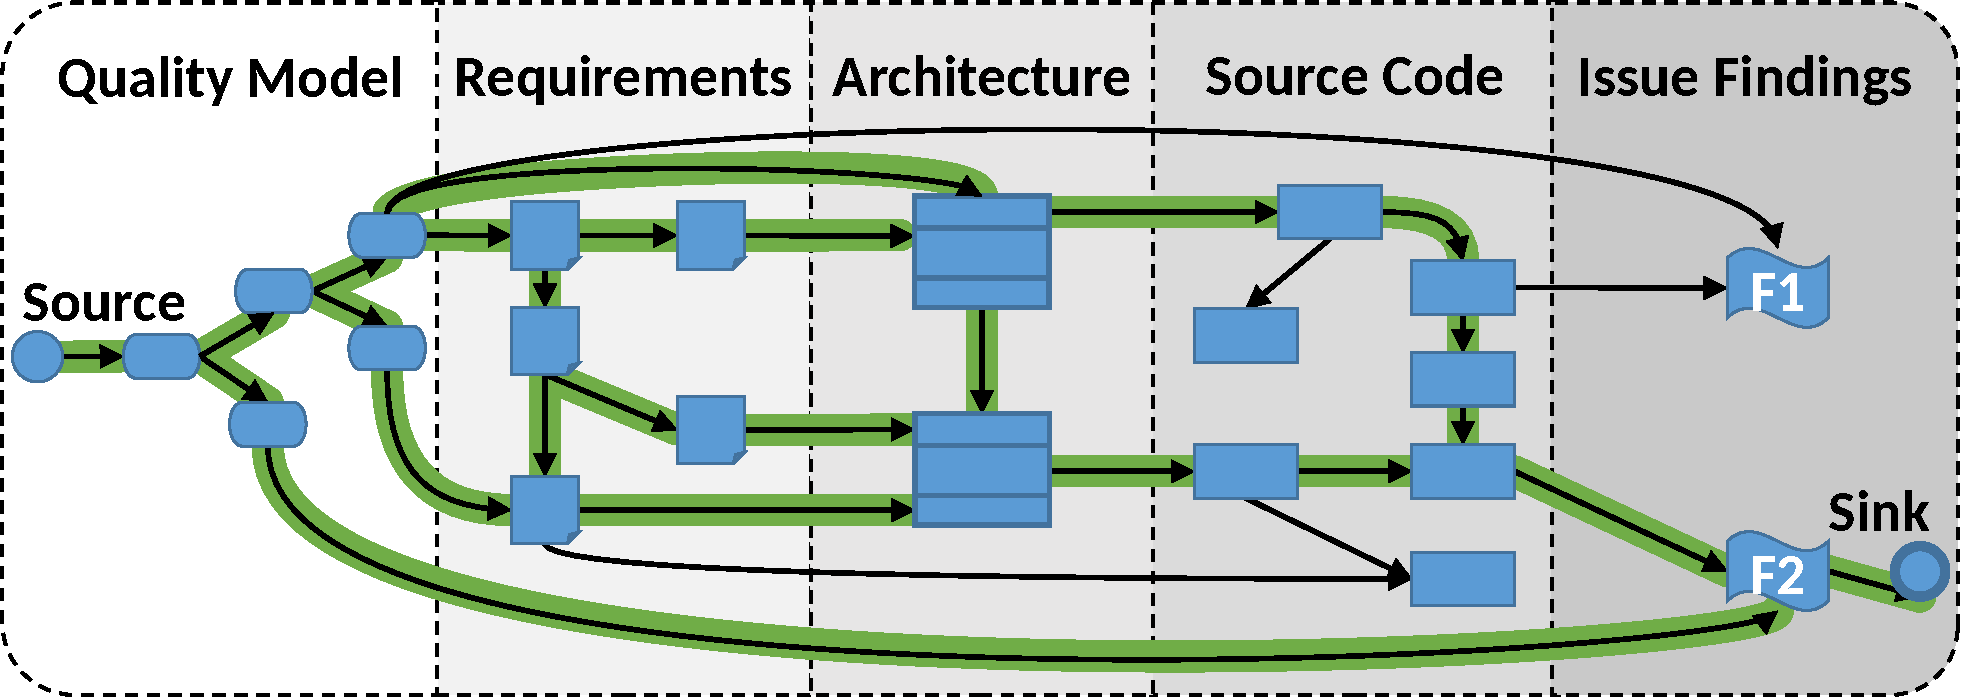
\includegraphics[width=.7\columnwidth]{figures/traces04-KG}%width=0.8\textwidth
	\caption{Example Flow Network with Typical Development Artifacts and Highlighted Flow for Issue F2}%Analysis
	\label{fig:traces}
\end{figure}

    \textbf{Aspect 1: Location of the issue.} The subsequent artifacts, such as requirements or design models, contain further knowledge about relations that \appr{} leverages for prioritization.
	For example, in practice issues may be identified in locations in the implementation that are differently connected to the rest of the code.
	Features such as logging are crosscutting and easily touch many parts of the implementation.
	Therefore, only considering flow within the implementation would over prioritize such issues.
	However, such features are only contained in planning artifacts such as design model if they are important for the project.
	By including such artifacts in the flow network, we can effectively prioritize issues.
	For example, not all nodes representing the source code in \autoref{fig:traces} are immediately connected with the requirements or design, therefore preventing direct flows towards them, lowering the total number of flow tokens that can reach issues detected on them.

    \looseness=-1
	\textbf{Aspect 2: Manual considerations.} In addition, trace links explicitly defined by security engineers or other stakeholders indicate a particular importance of the elements that are connected for the project.
	Accordingly, this could indicate that issues touching one of these elements are of higher importance.
	For example, consider an security engineer performing threat modeling on the architecture and reasoning about which threat categories, i.e., the ones of STRIDE\,\cite{STRIDE,Shostack2008}, might apply to specific elements in the architecture.
	If a possible threat is identified, this is documented whereby the threat categories considered are usually part of the quality model and it is documented to which design element this threat might apply.
	In the end, this results in a direct trace link from the quality model to the system model used at threat modeling, such as the link on top of \autoref{fig:traces} between the quality model and the architecture.
	Since these trace links lead to more edges in the flow network, it is possible to immediately propagate more flow tokens between them, therefore most likely increasing the number of flow tokens that reach an issue touching these elements, i.e., its priority.

	\textbf{Aspect 3: Security impact.} Lastly, analyzer detection rules usually indicate which quality aspects can be negatively affected by an issue detected by a particular rule, e.g., by relating the rule to common weaknesses from the CWE or listing aspects such as availability.
	These information is also embedded into the flow network and therefore considered in the prioritization.
	For example, in \autoref{fig:traces} as well F1 as F2 are immediately connected to nodes from the quality model.
%In this section, we show
%
%\begin{enumerate}
%    \item how software development artifacts connected by trace links can be converted into a flow network,
%    \item how the edges of this flow network can be weighted based on the importance of relations within the development artifacts and the relevance of the single trace links, and
%    \item how the importance of an issue can be quantified by solving the maximum flow problem for the issue.
%\end{enumerate}
%
Since prioritization using a maximum flow algorithm is straightforward after flow network construction, we focus on flow network construction.
First, in \autoref{DevArt}, we discuss which software development artifacts and trace links can be considered when constructing a flow network.
Except for a quality model, we do not give a fixed list of artifacts that must be considered, or those that are only supported by \appr{}, but discuss possible categories of artifacts, each with a concrete example using the Electronics Health Records system \emph{iTrust}\,\cite{iTrust} as running example.
For the quality model required by \appr{}, we discuss lightweight ways to obtain one.
We then show how such artifacts can be transformed into a flow network in \autoref{sec:flownetwork}.
Finally, in \autoref{sec:dsl}, we discuss in detail how arbitrary artifacts can be supported and their characteristics important for proper prioritization, such as the different types of relationships discussed above, can be reflected as weights of the edges in the flow network.
%\end{enumerate}

\subsection{Development Artifacts and Assumptions}
\label{DevArt}
%
\appr{} exploits trace links among various development artifacts that are usually created during the development of security-critical systems.
Within this paper, we assume traceability to be given such as required by many standards, e.g., the ISO/IEC 62304 for medical device software\,\cite{IEC62304}.
Existing work already investigates how to create and maintain trace links (for some approaches, see \autoref{sec:background:tracelinks}).

While conceptually \appr{} can be used with many different types of artifacts, here we describe those that we consider in the evaluation of our approach due to pragmatic reasons: Besides a quality model, they are already available for many software systems, as they are required by standards such as the ISO/IEC 62304\,\cite{IEC62304}.
Except for a quality model, they serve only as illustrative examples and developers are free to use other types of models, programming languages, or analyzers.
We describe them in the context of a running example, the \emph{iTrust} Electronics Health Records system \cite{heckman2018}.
The system has been developed as a class project at the North Carolina State University using Java and Java Server Pages~(JSP) and is repeatedly used in traceability and requirements engineering research\,\cite{zogaan2017datasets,MOHA2010,BSGRJS2018,Peldszus2019SDF,PBKJ2021,TPS2022}.


\subsubsection{Quality Model}

\begin{figure}
	\centering
	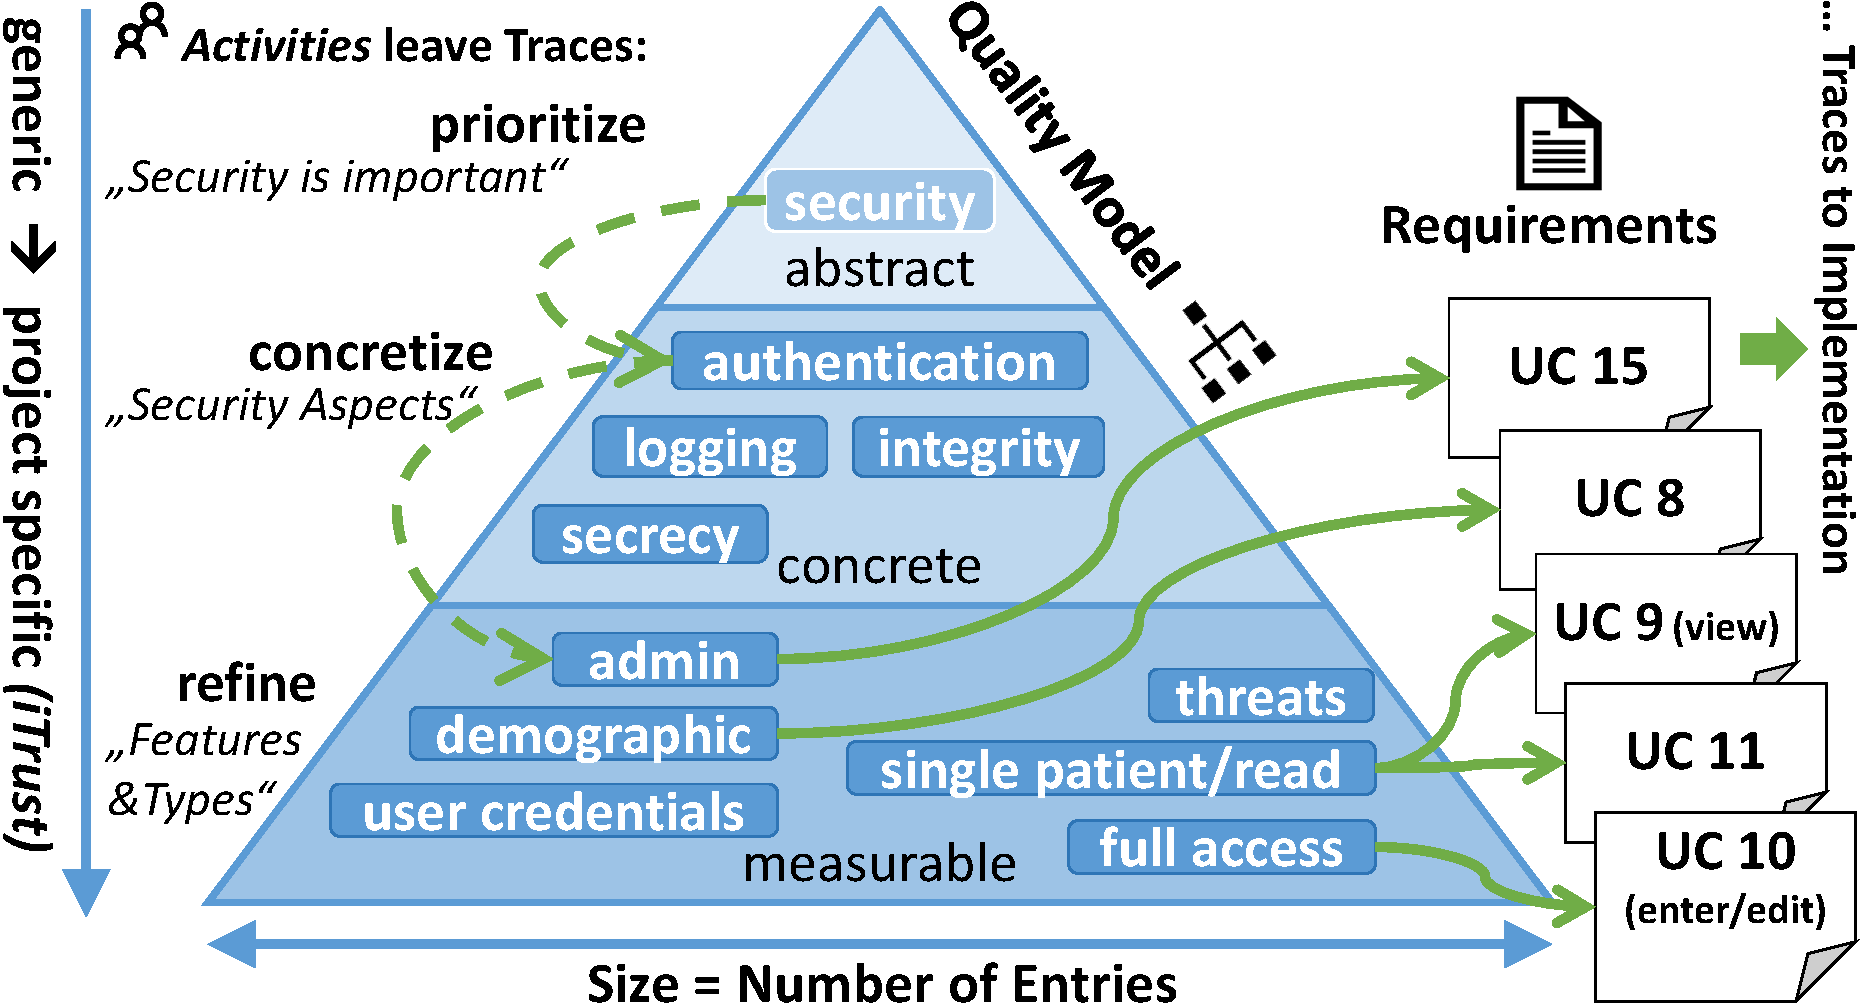
\includegraphics[width=0.7\columnwidth]{figures/QM}%0.8\textwidth
	\caption{%Refining
	Security Priorities in iTrust's Quality Model}
	\label{fig:qmodel}
\end{figure}

% Was ist ein QM?
A quality model captures, documents, and prioritizes quality aspects considered relevant for a particular project.
It is established by selecting important general quality aspects and refining them to concrete security features\,\cite{wagner2009security}.
Therefore, quality models exceed the abstract quality goals from ISO\,25010\,\cite{ISO25010,Schneider2012ASQ,WAGNER2015101}.

% Wie erstellt man ein QM im Kontext von TraceSec?
When establishing a quality model, stakeholders discuss and identify concrete, project-specific quality aspects. First, they prioritize generic qualities on an abstract level.
Next, the qualities are \emph{concretized} to relevant aspects of that quality.
This is crucial since it is an expression of a selection decision and a prioritization, which are considered indicators for relevance in \appr.
In the \emph{refinement} step, they refine types of features, affected data, or threats.
Finally, since different qualities are often seen to be of different importance to the project\,\cite{Wagner2012}, the stakeholders prioritize all quality aspects.
In particular, these different priorities of qualities need to be considered when later prioritizing issues in terms of their impact on the security of a project, since different vulnerabilities are likely to threaten different qualities.

	A quality model is the only required artifact in \appr{}.
	By considering a quality model as the reference according to which issues will be prioritized, we can capture arbitrary security aspects, such as confidentiality, integrity, privacy, or availability.
	Any relevant aspect can be captured in the quality model and will be considered in the issue prioritization.
	Thereby, different priorities of quality aspects will also be considered.

Since we consider the prioritization of security-related qualities in the quality model as the reference for relevance, \appr{} requires trace links between the quality model and subsequent artifacts, such as requirements (see \autoref{fig:qmodel}).
All downstream requirements, models, and implementations inherit their relevance from the quality model along the trace links.
While stakeholder priorities are discussed and documented in the quality model, trace links are created as a by-product of development activities.



% Wie sieht das im Running Example aus?
\autoref{fig:qmodel} shows a quality model excerpt for iTrust. %our running example.
%Since iTrust as a
Since the health application is built around the quality aspect of \emph{trust}, we assume security as quality to be of high priority.
Therefore, \emph{security} is selected at the most abstract level in \autoref{fig:qmodel}.
To demonstrate \appr{}, we look at security only, although usability or other quality aspects could be treated equally.
This is, however, beyond the scope of this paper. % which is purely focused on security issues.
In the concretization step, we identified security-related aspects of \emph{authentication}, \emph{logging}, \emph{secrecy}, and \emph{integrity} and created links to the quality aspect \emph{security}.
In the refinement step, we identified measurable units.
For example, access to purely \emph{administrative data} is considered less security-relevant than \emph{single-patient data}.
Trace links are then used to connect each quality to relevant elements from other development artifacts, such as related requirements in \autoref{fig:qmodel}.

% A quality model captures, documents, and prioritizes quality aspects considered relevant for a particular project.
% It is established by selecting important quality aspects and refining them to concrete features or non-functional requirements.
% \edit{Therefore quality models exceed} the abstract set of quality goals %requirements
% from ISO~25~010\,\cite{ISO25010,Schneider2012ASQ,WAGNER2015101}.
% %For example,
% %E.g., \emph{functional suitability}, \emph{usability}, \emph{performance efficiency}, \emph{portability}, \emph{compatibility}, \emph{reliability}, \emph{maintainability}, and \emph{security} are the top-level quality aspects in ISO~25~010\,\cite{ISO25010}. Stakeholders can use this abstract %quality
% %model %in ISO~25~010
% %to prioritize quality aspects for a given %software
% %project.

% \edit{\autoref{fig:qmodel} shows an excerpt of a quality model for our running example.}
% %\edit{For example,
% Since iTrust as a health application is built around the quality aspect of \emph{trust}, we assume security \edit{as quality} to be of high priority. %in the iTrust project,
% %if such a quality model would have been created %in the iTrust project.
% %for it.
% To this end, \emph{security} is selected on the most abstract level in \autoref{fig:qmodel}.
% To demonstrate \appr, we %will
% look at security only, although usability or other quality aspects could be treated
% equally. %accordingly.
% This analogy, however, is beyond the scope of this paper which is purely focused on security~issues.

% When establishing a quality model, stakeholders %and requirements engineers %would
% discuss and identify concrete\edit{, project-specific aspects of security, that they consider of particular importance.}
% In our running example (\autoref{fig:qmodel}), these include \edit{the security-related aspects of} \emph{authentication}, \emph{logging}, \emph{secrecy}, and \emph{integrity}.
% It is crucial to trace the refinement process \edit{since it is an expression of a selection decision and a prioritization, that are considered as indicators for relevance in \appr}.
% %We follow these choices as indicators of relevance.
% %There are several possible ways of tracing this refinement.
% \textcolor{red}{\todo{remove?}For example, one can create trace links from a refined aspect to all refining security aspects%after the refinement session
% , which can be done manually or supported by a tool.} %from security in general down to sub-aspects of security.
% In the next refinement step, \edit{and trace again)} %the
% types of features, affected data, or %potential
% threats.
% \edit{In the end, the stakeholder prioritize all quality aspects.
% We consider them the reference for relevance.}
% For example, access to purely \emph{administrative data} is considered less security-relevant %~(1)
% than \emph{single-patient data} access%~(4)
% %, or even \emph{full access} to all patient records%~(5)
% .

% %Concrete use cases or features may fall into one of those classes of security-relatedness.
% %Issues referring to high-score features will be considered more important than features that have nothing to do with security.
% \edit{\appr{} requires trace links between the quality model and requirements (see \autoref{fig:qmodel})}.
% %In \autoref{fig:qmodel}, %use cases and requirements are traced to relevant qualities\edit{, which can} occur during development, or %as a result of through reviews, %ing use cases later, as we did for iTrust.
% %In this paper, we assume those traces have been established in one way or another. %One can use traditional ways of tracing; we are also investigating techniques to facilitate creating traces. This aspect is discussed elsewhere.
% %
% %Fine-grained decisions along the process of creating the quality model lead to requirements. We consider these decisions and rationale  parts of the quality model. Requirements and use cases derived from those decisions are considered separate artifacts.
% %
% All downstream requirements, models, and implementations inherit their %importance and
% relevance from the quality model %---%and
% along the \edit{trace links}.
% \edit{
%     While stakeholder priorities are discussed and documented in the quality model, trace links are created as a by-product of those development activities. %The sequence of activities (i.e., reading a UML model, then writing a piece of code) can be traced manually, through commit messages, or in a dedicated editor.
% }
% %We map the propagation of importance from a quality model to implementations and warnings or issues to the maximum-flow model depicted in \autoref{fig:traces}. Importance flows along the traces from quality priorities %(in the quality model)
% %to requirements closely related to those high-priority quality aspects, down to model and code implementing those same requirements.

\subsubsection{Requirements}



As requirements are documented in various forms, from textual to formal models, to effectively exploit traceability information, it is recommendable to use a model focused on their trace links %, which abstract
and abstracts
from the actual notation.
For this, we use in our example a simplified adaption of \emph{T-Reqs}\,\cite{Grosser2022RDR}, that represents requirements and flows in a model-based fashion.
This allows us to reference requirements and their flows with trace links.

In the running example iTrust, the requirements are specified in 79 use cases, 36 of which are implemented in version 21 of iTrust.
Each use case is documented textually on an individual wiki page\,\cite{iTrustWiki}.
E.g., use case UC26 (see \autoref{fig:uc26}) describes the management of laboratory procedures by Health Care Personnel (HCP).
%\figurename~\ref{fig:uc26}  shows an excerpt of the model, we derived
We automatically derived a requirement model
%from this %textual representation
to obtain individual requirement objects and relations. % among them. %which can be used for our approach.
%The requirement metamodel with set-containment and typed relations is a simplified adaption of the \emph{T-Reqs} model\,\cite{Grosser2022RDR}.
For this, we extracted containment relations from the given section structure and additional trace information from hyperlinks and text labels, as illustrated in \autoref{fig:uc26}.
%
%\begin{figure*}
%	\centering
%	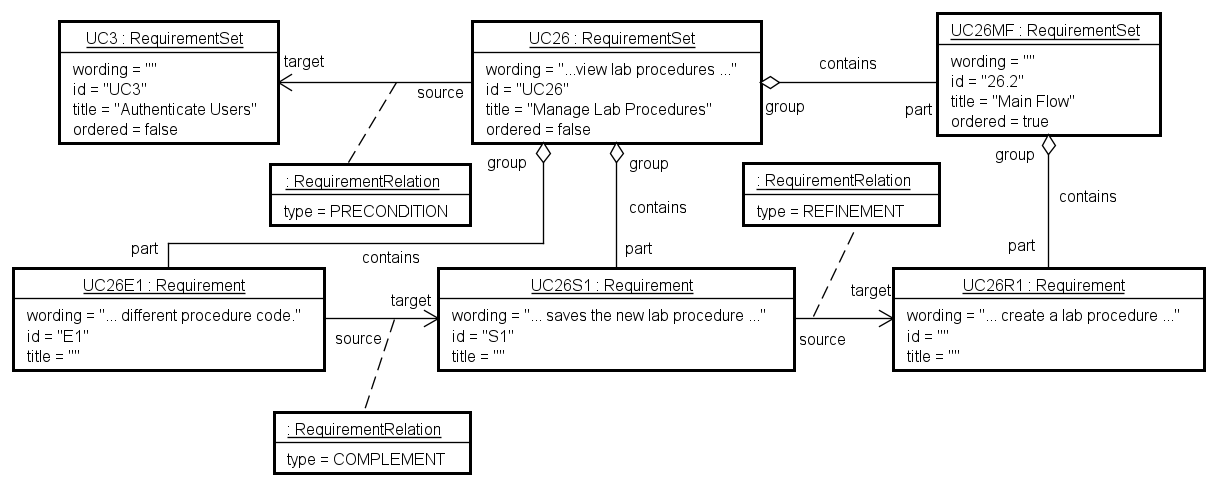
\includegraphics[width=0.8\textwidth]{figures/UC26_Objectdiagramm_wide.png}
%	\caption{Excerpt of Requiremets Model for iTrust UC26}
%	\label{fig:uc26}
%\end{figure*}
%
For example, UC26 contains the pre\-condition that requires the users to authenticate themselves (linking to use case UC3).
%The
A main flow section, consists of individual requirements, describes the general sequence of actions, %. %\autoref{fig:uc26} shows the main flow with its first requirement, describing lab procedure creation. As most main-flow requirements, it is
%This can be
and is refined by more detailed sub-flows. %, the requirement with ID \enquote{S1}.
Alternative flows describe actions with complementary conditions, e.g., deficient inputs. %, and are referenced from main or sub-flows. %S1 is complemented by the requirement \enquote{E1}. UC26 contains further sub and alternative flow requirements, as well as
Use cases contain additional requirements for logging events and links to other use~cases. %, not depicted in \figurename~\ref{fig:uc26}.

\begin{figure}
	\centering
	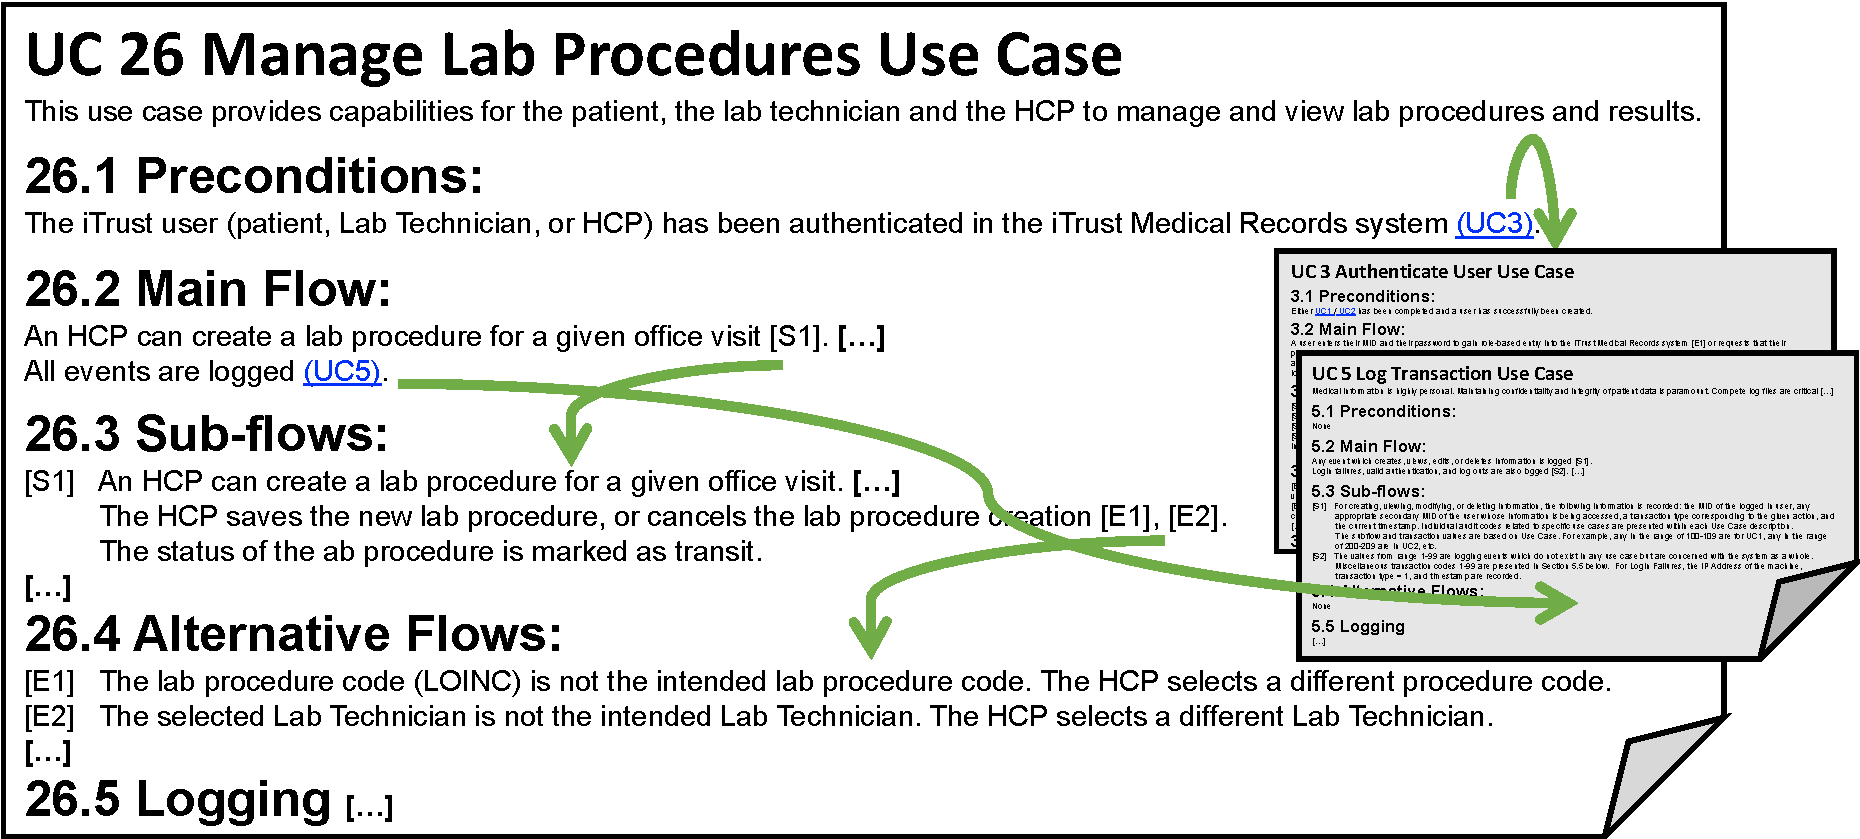
\includegraphics[width=0.9\columnwidth]{figures/UCexample2}
	\caption{Excerpt of iTrust UC26 and its dependencies; HCP = Health Care Personnel}
	\label{fig:uc26}
\end{figure}

\subsubsection{Architecture}

\begin{figure}
	\centering
	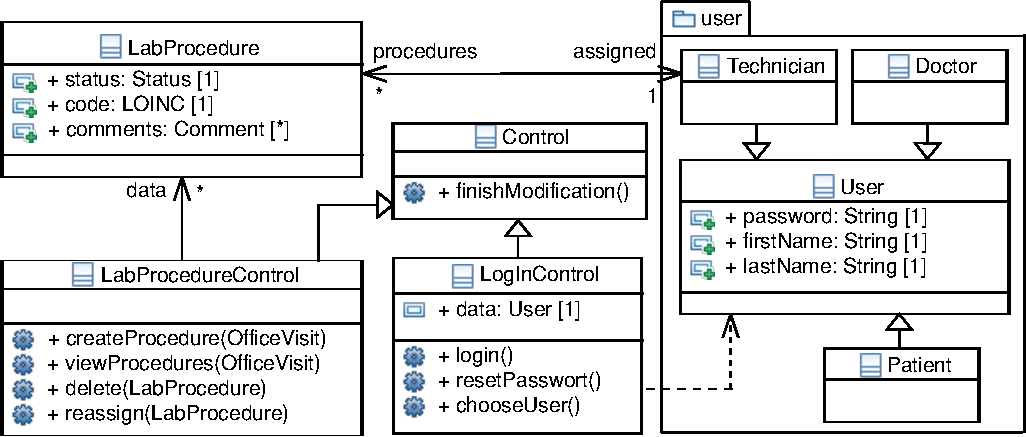
\includegraphics[width=.75\columnwidth]{figures/itrust-classdiagram-labprocedure.pdf}%0.8\textwidth
	\caption{Excerpt from the iTrust Class Architecture}% of the iTrust System
	\label{fig:clsarch}
\end{figure}

At systems development, architecture specifications should express the fundamental relationships among architectural elements and are a mean for planning and documenting the system implementation\,\cite{CGL+03}.
In \appr{} we support model-based rep\-resentation of the major structural elements and their interrelations as architecture specification, e.g., component-and-connector views\,\cite{Ivers2004DCC,Bertram2017}.
If architectural models are used, we need the architectural structures to relate structural elements to the requirements and the quality model.
In this way, we specify which structural elements are particularly relevant for the quality goals.

While \appr{} allows for any or even multiple architecture description languages, in the running example, we use an architecture specification utilizing the Unified Modeling Language (UML),
a widespread standard for specifying software architectures\,\cite{uml}.
In various works, UML models specifying the architecture of iTrust have been reverse-engineered\,\cite{MOHA2010,BSGRJS2018,PBKJ2021}.
%In this work, we are using these as architecture specifications in our evaluation. %as well as for the introduction of the iTrust system’s architecture.
%
The requirements of iTrust are realized by \emph{Control} classes for each use case, complemented by classes for data.

\autoref{fig:clsarch} shows an excerpt from the class architecture showing these controls and classes representing users of the system:
%
The class \textit{LaboratoryProcedureControl} realizes the management of laboratory procedures as specified in UC26, while \textit{LoginControl} realizes the required authentication as described in UC3. For all classes, essential data and functionality is specified as properties and operations. %These are going to be detailed and realized in the implementation.

	In practice, the design may not map as conveniently to the requirements.
	Nevertheless, the software architects usually develop a system design having the requirements at hand, thereby manually recording trace links.
	In the end, providing at least some traceability is unavoidable, since developers are assigned tasks to implement specific requirements at a given location in the system design.
	This information is usually provided more or less explicitly, e.g., via ticket systems.
	If not provided, developers have to manually search for the corresponding locations in the system and should document this information.
	As briefly discussed in \autoref{sec:background:tracelinks}, there also exist approaches for automated trace link retrieval between requirements and architecture\,\cite{Goknil2014,Keim2024}.

\subsubsection{Threat modeling}
Threat modeling is a technique to systematically identify possible threats to the system under development\,\cite{Shostack2008}.
In popular threat modeling approaches such as STRIDE\,\cite{STRIDE,Shostack2008} or PASTA\,\cite{pasta}, the system is represented at a coarse-grained level to allow systematic reasoning about possible threats to the system.
A common representation used for this purpose is data flow diagrams, but any abstract system model could be used, e.g., UML models defining an abstract system design.

Based on these diagrams, security experts reason about possible threats for each element in the diagram. Frameworks such as STRIDE assist the experts by providing types of threats that can compromise the security of a system. STRIDE itself is an acronym that stands for the categories that need to be considered: Spoofing, Tampering, Repudiation, Information Disclosure, Denial of Service, and Elevation of Privilege.

Ultimately, these types of threats comprise qualities that are expressed in the quality model, i.e., an instance of the threat of spoofing would threaten the quality ``authenticity'' shown in \autoref{fig:qmodel}.
The considered threat types are documented in the quality model as qualities, possibly accompanied by custom project-specific qualities.
When security experts reason about and document threats in the system representations, this information can be used as trace links from the quality model to the design models inspected during threat modeling.
	Each identified threat results in an explicit trace link between the threatened design element and the threat, i.e., quality from the quality model.
	For example, the direct edge between the quality model and the architecture in \autoref{fig:traces} results from such a trace link.

In the case of limited resources, only the qualities of the selected threat model can be considered to manifest a quality model.
For STRIDE, the quality model would merely consist out of the six threat categories, which could be ranked according to project needs or be considered as equally important.

In addition to STRIDE, there are several other threat modeling frameworks that provide different types of threats that can be considered.
For example, LINDDUN\,\cite{deng2011privacy} provides threats tailored to privacy. When several of these frameworks are used, the quality model serves as a means to relate them.

\subsubsection{Source Code}
\appr{} needs the program code as a processable model at an appropriate level of abstraction.
We need knowledge about containment relationships (e.g., classes in a package, methods in a class) as well as cross-references (which method calls which other method).
Various tooling, such as MoDisco \cite{modisco} or JaMoPP \cite{jamopp}, exists to extract such models from source code written in specific programming languages, i.e., Java.
However, while these tools resolve references such as method calls, these usually contain all details from the statement level, leading to huge models.
We use the GRaViTY program model\,\cite{PKLS2015,Peldszus2022,Peldszus2024} for making this information accessible.
%For the analysis of the system’s source code, we use the GRaViTY program model\,\cite{PKLS2015,Peldszus2022}.
The program model provides an abstraction from the fine-grained abstract syntax tree reducing details from the statement level of methods and fields to explicit dependencies between these, e.g., calls between class members.
This abstraction allows considering fewer details %on the statement level
of the implementation, i.e., 28\% fewer nodes than a MoDisco model \cite{Peldszus2024}, when prioritizing issues, which reduces the size of the flow network and improves the run-time overhead.
Finally, the GRaViTY model is designed to support arbitrary object-oriented programming languages \cite{PKLS2015}, therefore providing the flexibility to support further programming languages besides Java.

\autoref{fig:javaiTrust} shows an excerpt of the program model extracted from the running example's source code focusing on the edit of a lab procedure implementing the class \textit{LaboratoryProcedureControl} from the class design in \autoref{fig:clsarch}.
The excerpt focuses on the addition of a comment to a laboratory procedure through a \textit{LabProcedureForm}, which is one of the classes realizing the \textit{LabProcedure} from the class design, using its method \textit{addCommentary}.
Adding a comment includes various calls to other functionality such as \textit{edit} to update the status that is stored in the field \textit{labProcedureStatus}.

\begin{figure}
	\centering
	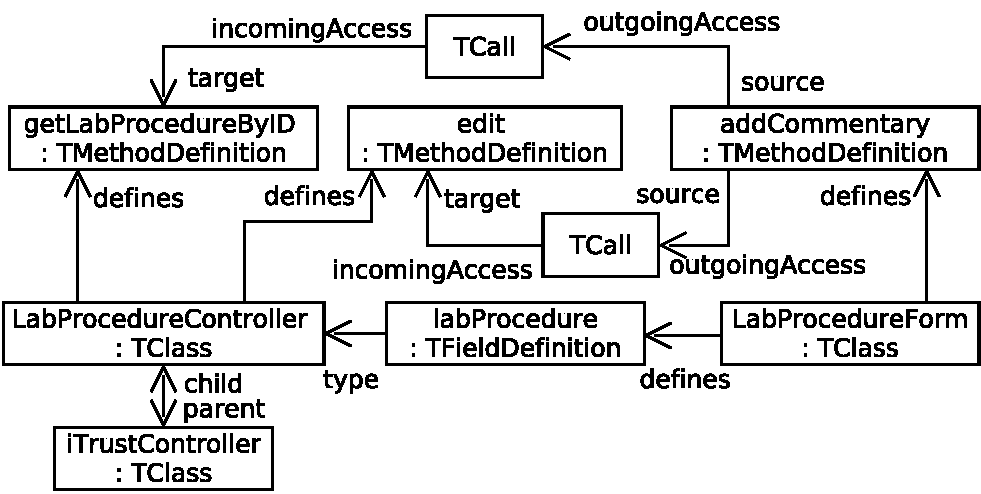
\includegraphics[width=.65\columnwidth]{figures/java-itrust-editLabProcedure}%0.8\textwidth
	\caption{Excerpt from the iTrust Program Model}
	%\caption{Excerpt from the Program Model of the iTrust System showing the Edit of a Lab Procedure}
	\label{fig:javaiTrust}
\end{figure}

\subsubsection{Issues}
Many analyzers, such  as SonarQube\,\cite{sonar}, SpotBugs\,\cite{SpotBugs}, PMD\,\cite{pmd}, CodeQL\,\cite{codeql}, and many others, analyze source code for implementation issues.
To do this, these analyzers typically rely on detection rules that express known violation patterns.
These weaknesses expressed in the rules can usually be immediately related to qualities from the quality model.
Since all of these analyzers detect concrete vulnerable code statements, we assume that issues in \appr{} are always related to concrete code locations, and optionally have further relationships to quality aspects that are threatened by the type of issue.

\looseness=-1
In this work, we compute issues with SonarQube, but any other static analysis tool will work.
Therefore, the following describes how to integrate an analyzer into \appr{}, using SonarQube as an example.
Just as the elements from all other models, issues detected by SonarQube must be connected with all relevant elements, i.e., the code location at which the issue has been detected or affected qualities in the quality model, via trace links.
To realize the necessary trace links to the source code, we use an extension mechanism of GRaViTY\,\cite{peldszus2016continuous} and annotate program model elements with the issues. To navigate to the lines of code where the issues are located, we keep a reference to the file and line.
%to add them directly as annotations.
Furthermore, SonarQube’s detection rules can contain references to relevant security aspects, e.g., when the issue targets a concrete weakness, e.g., one of these captured in the common weakness enumeration (CWE)\,\cite{cwe}, further underlining their importance.
%For example,
In the running example, the two issues in \autoref{fig:traces} are vulnerabilities directly threatening a security aspect in the quality model. Nevertheless, based on their location in the code, they do not have the same priority.

\subsection{Converting Artifacts into a Flow Network}
\label{sec:flownetwork}
%
%The first problem we have to solve if we want to calculate the maximum possible flow through a network from a source to a number of sinks is the creation of this network.
%In our case, the sinks are the findings of static analyzers, the network is given by the trace links and dependencies within the development artifacts, and the source is the root of the quality model.
%In what follows, we describe in detail how to create a flow network from the development artifacts of a software project and trace links between these.
%
%Traces indicate references to previously developed elements and therefore build the connection between the different artifacts.
To create a flow network (step 2 in \autoref{fig:PrioApproach}), we assume that every trace link can contribute to the importance of an element and
thus
is %therefore
represented by an edge in the flow network. As we %are going to
propagate importance from the quality model to the findings, we assume every edge derived from a trace link to point in this direction. All elements connected by trace links become nodes of our flow~network.

Nodes added to the flow network based on trace links may also be interconnected via relations within the development artifacts.
%The nodes added to the flow network based on the trace links may also be connected through relations within the single development artifacts.
For example, two classes linked by trace links may be in an inheritance relationship.
Such relations also contribute to the flow network as edges.
The new element and its relations are added to the flow network recursively to include all potentially relevant elements and relations.
Finally, we get an iterative construction algorithm that terminates when there are no more relations to~process.

\begin{algorithm}
        \caption{Flow Network Creation}
        \label{algo}
		\SetKwInOut{Input}{Input}
		\SetKwInOut{Output}{Output}

		\Input{Set of Trace Links \emph{traces}, Quality Model \emph{qm}}
		\Output{Flow Network G(\emph{nodes}, \emph{flows})}
		\BlankLine
		stack := \{qm$\rightarrow$allRelations()\}\;
		flows := \{\}\;
		nodes := \{node(qm)\}\;
		\BlankLine

		\ForEach{t $\in$ traces}{
			src := nodes$\rightarrow$getOrCreate(t.src)\;
			trg := nodes$\rightarrow$getOrCreate(t.trg)\;
			flows$\rightarrow$add(src, trg, capacity(src, trg))\;
			stack$\rightarrow$addAll(t.src$\rightarrow$allRelations())\;
			stack$\rightarrow$addAll(t.trg$\rightarrow$allRelations())\;
		}
		\BlankLine
		seen := \{\}\;
		\While{stack$\rightarrow$hasNext()}{
			relation := stack$\rightarrow$pop()\;
			\BlankLine
			\If{!seen$\rightarrow$contains(relation) \&\& consider(relation)}{
				seen$\rightarrow$add(realtion)\;
				src := nodes$\rightarrow$getOrCreate(relation.src)\;
				trg := nodes$\rightarrow$getOrCreate(relation.trg)\;
				flows$\rightarrow$add(src, trg, capacity(src, trg))\;
				stack$\rightarrow$addAll(relation.trg$\rightarrow$allRelations())\;
			}
		}
\end{algorithm}

\autoref{algo} shows how the flow network can be created, considering trace links and the relations within single artifacts.
The algorithm takes a set of trace links among the development artifacts and a quality model as input.
%a quality model and all trace links among the development artifacts and returns a flow network.
In lines 1--3, data structures for building the network are initialized.
These comprise sets of all nodes and all flows in the constructed flow network and a \texttt{stack} for storing relations among development artifact elements that have to be processed.
To guarantee that the entire quality model will be added to the flow network, the set of \texttt{nodes} is initialized with a node representing the root of the quality model, and the stack of unprocessed references is initialized with all outgoing references.
First, we iterate over all trace links in lines 4--10 and add flows expressing each trace link to the flow network.
In lines 5--6, we retrieve the nodes corresponding to the trace link's source and target or create corresponding nodes if the element has not been processed yet, using a helper function \texttt{getOrCreate}.
Afterward, we add an edge between these two nodes to the flow network (line~7).
Here, we also calculate the edge's capacity (see \autoref{edgeCap}).
In lines 8--9, we add all outgoing relations of the trace link's source and target to the stack of unprocessed relations for being processed after all trace links have been processed.

After leaving the loop in line 4, all trace links are represented by edges in the flow network but the connections within the different artifacts are missing.
Starting from line~11, we add these additional elements to the flow network.
To avoid adding edges twice, we first initialize a stack containing all relations that have been processed (\texttt{seen}).
Afterward, in lines 12--21, we process all  references that have been put on the reference \texttt{stack}.
According to  line 14, we add a reference to the flow network if it has not been added before (not being on the \texttt{seen} stack) and the relation is not ignored by the user (see \autoref{edgeCap}).
For determining if a relation is not ignored and therefore should be considered, we use a helper function \texttt{consider} that will be explained afterward.
If a relation is to be added, we first put it on the stack of seen references and proceed as we did for the trace links.
As the target of the reference might contain references that have not been considered yet, we add all outgoing references to the relation stack.
Once the relation stack is empty, the flow network has been constructed successfully.

At network construction, we want to only consider the relation types that contribute to propagating importance.
%As not every kind of relation contributes to propagating importance, we only consider the kinds of relations that can do so.
This filtering allows us to create flow networks faster and reduces the effort of solving the maximum flow problem as the flow network will be smaller.
%In the next section,
Next, we introduce how this filtering can be tailored towards concrete projects and how edge capacities will be determined.

\subsection{Filtering and Determining Edge Capacities}\label{edgeCap}
\label{sec:dsl}
%
\noindent
In \appr{}, we aim to support arbitrary artifacts created during development.
Besides those considered in our example, common artifacts include data flow diagrams (DFD) for threat modeling\,\cite{Shostack2008,TUMA2018275}, business process models (BPMN)\,\cite{white2008bpmn}, Palladio component models\,\cite{reussner2011palladio}, other, perhaps even security-specific, requirements models\,\cite{8004340}, and many others.
For each of these model types, it is necessary to specify how to integrate them into a flow network.
Furthermore, it may even be project-specific which elements to consider and how to consider them.
For this reason, it is not possible to integrate this logic directly into the network construction.
To this end, we allow an exchangeable and reusable artifact import specification of what should be considered when constructing the flow network, allowing even project-specific considerations to be taken into account.
To achieve this, we have specified a domain-specific language (DSL)\,\cite{fowler2010domain,dsl} that allows specifying not only which reference types should be included, but also which capacities should be assigned to the corresponding edges in the flow network.
This DSL allows experts, such as maintainers of a particular modeling language, to specify artifact import specifications to support specific artifacts in prioritization.
Other security experts of companies using \appr{} can take these specifications and optimize them according to project characteristics, e.g., to optimize the created flow network by considering the level of detail in design models, the amount of available trace links, or to define metamodels for specific model types used in the project.
Afterwards, the prioritization can be performed by all developers without taking these details into account, just by using the provided configurations.
Our examples provide default settings for common artifact types.

Since the source of the maximum flow problem is the root of the quality model and the sink an issue in the implementation, we are searching for the maximum flow from the most coarse-grained element to one of the most fine-grained element.
Therefore, when adding edges to the flow network, we refine importance in the context of system refinement.
%Therefore, when adding edges to the flow network, the underlying assumption is that importance always flows \emph{from coarse-grained elements to fine-grained elements}.
If we would allow flows in the opposite direction, this would allow additional flows over entirely unrelated elements and therefore prevent proper prioritization.
For example, consider a flow from a requirement to an element in the system design that then propagates trough the design until it reaches an design element relevant to an additional unrelated requirement, which will eventually happen in every system unless it could be split into two independent systems.
This second requirements then has relations to additional parts of the implementation entirely unrelated to the first requirements but will allow flows that suggest an relation.
To this end, it is not necessary to explicitly specify the direction in which trace links should point or whether they should be considered, but only the order of the artifacts between which trace links exist.
In the construction algorithm, all trace links are added to the flow network and the direction is derived from the order of the artifacts.
It is also necessary to calculate the capacity with which they should be added.
For example, a direct trace from the quality model to the implementation is more important than a trace to the architecture, which should be reflected in the capacities.
In our approach, the capacity of edges representing trace links depends on the distance between the models, with the desired order specified by the user.
In our example, we assume the following order of artifacts (as in \autoref{fig:traces}):

\begin{small}
\begin{description}
\item \texttt{Quality Model (0) < Requirements (1) < Archi\-tec\-ture~(2) < Program Model~(3) < Findings~(4)}.
\end{description}
\end{small}

%Weights (represented as capacities in the flow network) express how heavily the different coarse-grained security aspects in the quality model are affected by a detected issue.
However, there is no explicit capacity assigned to each individual trace link---neither in a project nor in our approach.
%In this paper, we postulate the existence of those traces, no matter how they were created. Creating traces as a by-product of project activities is a separate line of work we conduct in parallel. It is beyond the scope of this paper.
We assume that every \emph{stage} is assigned with an increasing value allocated to the nodes representing entities from these development artifacts.
The concrete capacity of a flow edge representing a trace link is calculated by a customizable function \texttt{capacity(Node, Node)}, calculating the capacity based on the distance between the nodes.
For simplicity, we show a linear function that only adds a static configuration factor for adjustment, e.g., selected depending on how intensively trace links are created within a project:

\begin{small}
\begin{description}
\item
\texttt{capacity(Node a, Node b): abs(a.stage-b.stage) $\times$ factor}.
\end{description}
\end{small}

In addition to direct trace links between elements of individual artifacts, there are also indirect trace links, such as through inheritance or containment relationships within an artifact.
To this end, besides trace links, we have to consider different edge types from the models: % in our flow network:
%First, there are edges whose capacity can be determined based on their type, e.g., inheritance or refinement links.
%Second, there are also edges whose capacity should be determined based on the concrete model instance:

\begin{enumerate}[label=\alph*)]
    \item To allow the customization of quality relevance, in the quality model custom priorities can be specified.
    These priorities should be reflected as capacities of the flow edges pointing to the nodes representing a quality.
    \item In all other models, the capacities are not specified individually %based on the concrete instances
    for each instance but the considered relationship types are associated with capacities.
    %These capacities can be statically specified using a configuration file.
    E.g., one can assume that every flow edge created for a \textit{Generalization} will have the capacity 1 and every \textit{Containment} %relation
    the capacity~2.
\end{enumerate}

How to handle these edges is specified in the proposed DSL.
While \autoref{lst:grammar} provides the syntax of the DSL, \autoref{dsl} shows an instance that contains exemplary specifications that make the metamodels of three artifact types used in the running example of this work accessible to \appr{}.
By using additional instances or by extending the shown one, arbitrary metamodels can be made accessible to \appr{}.
We explain the syntax of the DSL on the example.
The syntax itself is written in the Xtext\,\cite{xtext} language grammar, which is similar to the Extended Backus–Naur Form (EBNF)\,\cite{Yue2014}.

Each instance represents a \texttt{Configuration} that makes an arbitrary number of metamodels, e.g., for representing requirements or design models, accessible to \appr{}.
We assume that the metamodels are organized by \texttt{Namespace}s, as in the Eclipse Modeling Framework (EMF)\,\cite{steinberg2008emf, EMFBook}.
For each namespace, one can specify a default capacity for all references within the metamodel and whether all its elements should be considered by default or not.

For example, in lines 1--4 of \autoref{dsl}, in the artifact import specification for the UML metamodel, we specify that all elements should be included with a capacity of~2.
This is the simplest case needed to support an artifact type, i.e., all elements specified in its metamodel, in \appr{}.
These artifact import specifications may become more complicated, as our UML specification does, to reflect the characteristics of the modeling languages.
We will demonstrate this with the other two artifact import specifications shown in \autoref{dsl}.

For the GRaViTY program model, in lines 6--15, we include also all elements by default, but additionally, specify special handling of two elements.
For every namespace, one can specify which of the types that are defined in the metamodel should be included or excluded when building the flow network.
Again, in the grammar rule \texttt{Type}, the same default values as for namespaces could also be defined on the scope of single types.
Within a type, one can specify references that should be included or excluded.

\lstset{
    string=[d]{"},
    stringstyle=\color{blue}
}
\begin{lstlisting}[caption={Grammar of the DSL structured into multiple grammar rules}, label=lst:grammar, float, keywords={enum,INT,STRING},basicstyle=\small\ttfamily,breaklines]
Configuration:
  ("default" "=" default=INT)?
  ("consider" "=" consider=Consider)?
  (namespaces+=Namespace)+;

Namespace:
  "namespace" package=STRING "{"
    ("default" "=" default=INT)?
    ("consider" "=" consider=Consider)?
    ("include" "{" (include+=Type)* "}")?
    ("exclude" "{" (exclude+=[ecore::EClass])+ "}")?
  "}";

Type:
  "type" type=[ecore::EClass] "{"
    ("consider" "=" consider=Consider)?
    ("default" "=" default=INT)?
    ("include" "{" (inlcude+=Edge)+ "}")?
    ("exclude" "{" (exclude+=[ecore::EReference])+ "}")?
  "}";

Edge:
  "reference" reference=[ecore::EReference] ("--" type=[ecore::EClass]
    ("--" target=[ecore::EReference])?
  )? direction=Direction weight=Weight;

Weight: NumberWeight | AttributeWeight;
NumberWeight: value=INT;
AttributeWeight: value=[ecore::EAttribute];

enum Consider: ALL="ALL" | NONE="NONE";
enum Direction: FWD="->" | BWD="<-" | BI="<->";
\end{lstlisting}

%\vspace{-4pt}
%float,
\begin{lstlisting}[
    language=Java,
    basicstyle=\small\ttfamily,
    numbers=left,
    tabsize=1,
    breaklines=true,
    morekeywords={namespace,default,consider,include,type,reference,exclude},
    caption={Example for the use of the DSL for Specifying a Configuration for Creating the Flow Network},
    label=dsl,
    float
]
namespace "http://www.eclipse.org/uml2/5.0.0/UML" {
 default = 2
 consider = ALL
}

namespace "http://www.gravity-tool.org/typegraph/basic" {
 default = 2
 consider = ALL
 include {
  type TMember {
   include { reference accessing--TAccess--target -> 1 }
  }
 }
 exclude { type TAnnotation }
}

namespace "http://www.tracesec.org/qualitymodel" {
 consider = NONE
 include {
  type Quality {
   include { reference aspects--Aspect--quality -> priority }
  }
 }
}
\end{lstlisting}


%\begin{lstlisting}[
%    language=Java,
%    basicstyle=\footnotesize\ttfamily,
%    numbers=left,
%    tabsize=1,
%    breaklines=true,
%    morekeywords={namespace,default,consider,include,type,reference,exclude},
%    caption={Configuration for building the flow network},
%    label=dsl,
%    float
%]
%namespace "http://www.eclipse.org/uml2/5.0.0/UML" {
% default = 2
% consider = ALL
%}
%
%namespace "http://www.gravity-tool.org/typegraph/basic" {
% default = 2
% consider = ALL
% include {
  %type TMember {
%   include {
%    reference accessing--TAccess--target-> 1
%   }
%  }
% }
% exclude {
%  type TAnnotation
% }
%}
%
%namespace "http://www.tracesec.org/qualitymodel" {
% consider = NONE
% include {
%  type Quality {
%   include {
%    reference aspects--Aspect--quality-> priority
%   }
%  }
% }
%}
%\end{lstlisting}


For includes and sequences of references, we can specify the inclusion of references pointing only to certain types, and the capacity and direction of the corresponding edge in the flow network (cf. grammar rule \texttt{Edge}).
In lines 10--12, we specify how accesses between class members (\texttt{TMember}) are considered.
Instead of \texttt{TAccess} nodes, the pair of references \texttt{accessing} and \texttt{target} will be added as a single edge in the flow network.
Furthermore, the direction in which the edge will point in the flow network is specified (\texttt{->, <-, or <->}), in this case in the reading direction.
Finally, due to the usually high number of accesses in an implementation, we specify that the edges should only be considered with a capacity of 1 instead of the default value of 2, to allow a more fine-grained propagation of flow tokens.
While the purpose of this value mainly is to demonstrate the capabilities of the DSL, it still stems from an practical observation.
However, the concrete value should be determined based on long-term experiences.

%Finally, as in our example only annotations such as \textit{@Deprecated} are used, annotations have only a connection to the annotated element and cannot contribute to the flow network but will grow it unnecessarily, we exclude these in line~14.

As the last part of the artifact import specification for the GRaViTY program model, annotations are excluded in line 14.
Those used in the example implementations, such as \textit{@Deprecated}, only link to the annotated element and cannot contribute to the flow network, but will make it grow unnecessarily.
In the full specification for the program model, however, this exclusion of annotations is overridden by a more fine-grained specification that considers issue annotations, which are subtypes of \texttt{TAccess} and would otherwise also be excluded.


%\edit{We include no element from the quality model} by default but only those explicitly specified \edit{(only the nodes of type \texttt{Quality}).
%The user-defined priority of a \texttt{Quality} is defined on an \texttt{Aspect} node between the quality and its parent \texttt{Quality}.}
%As for the accesses among members, we do not add these nodes to the model.
%As the capacity of the resulting edge, we use the value stored in the attribute~\texttt{priority}.

We include only explicitly specified elements of the quality model (i.e., only the nodes of type \texttt{Quality}).
Like the accesses among members, we do not add these nodes to the model.
The user-defined priorities in the quality model, which should be considered as edge capacities, are defined in a \texttt{priority} attribute of an \texttt{Aspect} node.
This node relates two \texttt{Quality} nodes to each~other.

Using this DSL, experts can specify default values for the scope of namespaces and types.
Furthermore, specific elements can be explicitly excluded or included in the flow network construction.
Finally, for each reference type, a static capacity or a pointer to an attribute holding the capacity can be specified.
To the end user using the \appr{} issue prioritization, these specifications are black-boxes, and they use only the artifact import specifications that are provided to them by experts.
	While we show a concrete optimization based on a practical observation, we explicitly avoided detailed optimizations in this work.
	The configurations used in this work are as simple as those shown above and are still suitable to achieve proper prioritization.
	Therefore, the effort needed to support a different metamodel is as low as writing 4 lines as for the UML example shown in \autoref{dsl}.
	However, there is still an opportunity for detailed fine-tuning if needed, e.g., due to further observations similar to the one described.
%Finally, per included element a static capacity can be specified or a pointer to an attribute of the model instance.
\section{Tool Support}
\label{sec:tool}
\begin{figure}
    \centering
    \begin{subfigure}{.365\columnwidth}
    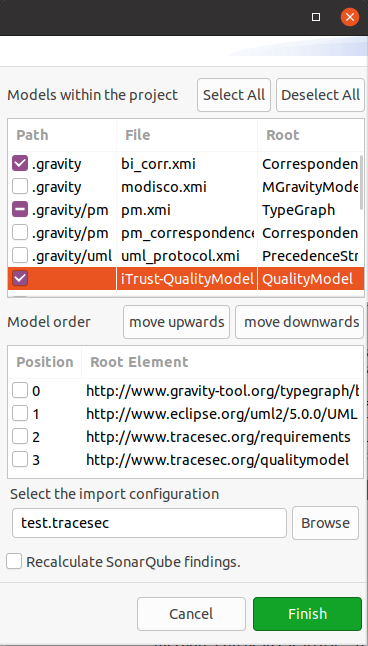
\includegraphics[width=\columnwidth]{figures/tracesec-impl-selection.png}
    \caption{Selection Wizard}
    \label{fig:wizard}
    \end{subfigure}
    \begin{subfigure}{.61\columnwidth}
    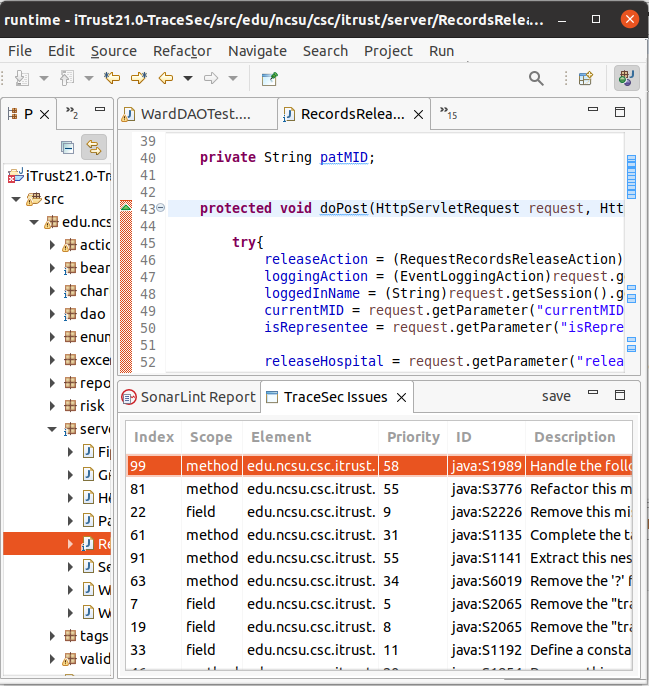
\includegraphics[width=\columnwidth]{figures/tracesec-impl-results.png}
    \caption{Result Presentation}
    \label{fig:results}
    \end{subfigure}
    \caption{Screenshots of the Tool Support}
    \label{fig:impl}
\end{figure}

We implemented \appr{} in Java with an Eclipse\,\cite{eclipse} plugin as a front-end for integration with the Eclipse IDE.
The tool introduces a wizard for calculating priorities for a Java project.
\autoref{fig:wizard} shows the UI of the wizard for selecting the models to be considered in the prioritization.
In the upper half, the user selects the quality model, the program model, models containing trace links, and other models to be considered, such as requirements or UML models.
The tool uses the Eclipse Modeling Framework (EMF)\,\cite{steinberg2008emf} for models.
In the lower half, the user arranges the selected models to define the order of the artifacts from which the tool calculates the distance between model elements needed to compute the flow in the flow network. In addition, the user specifies a configuration file that declares project specific capacities and ignores certain types of relationships using the DSL we provide, as shown in an example in~\autoref{dsl}.
The SonarQube issues are calculated (if not already present) and added as annotations to the program model.

The prioritization view (bottom of \autoref{fig:results}) shows the issue findings in a list view, giving details about their id, scope (\emph{class}, \emph{method}, or \emph{field}), location, issue description, and the priority as automatically calculated by \appr.
The table view allows navigating to each issue in the code on click.
%

To specify the artifact import specification using the DSL introduced in \autoref{sec:dsl}, we implemented this DSL using the language engineering toolkit  Xtext\,\cite{xtext}.
Given a grammar such as the one shown in \autoref{lst:grammar}, Xtext allows the generation of parsers and runtime editing support integrated into IDEs\,\cite{BPA+2022}.
Internally, Xtext is based on EMF for providing access to the parsed DSL instances, which allows explicitly referencing types from EMF-based metamodels, i.e, EMF-based implementations of the UML\,\cite{Gerard2007}, BPMN\,\cite{EclipseBPMN}, data flow diagrams (DFDs)\,\cite{Tuma2019}, or Palladio\,\cite{reussner2011palladio}.
In this way, the DSL allows immediate interaction with EMF models, including editing support such as auto-completion, even for elements specified in imported EMF metamodels, syntax highlighting, and validation.
Since Xtext supports the Language Server Protocol (LSP)\,\cite{lsp}, this editing support is not limited to the Eclipse IDE, but can serve any IDE that supports the LSP\,\cite{BPA+2022}.
We provide instances of this DSL (cf. \autoref{dsl}) to support the quality model used by \appr{}, requirements models based on a metamodel we created to capture the requirements of iTrust that is oriented on the requirements relation model of Großer et al.\,\cite{Grosser2022RDR}, UML models\,\cite{uml}, and the GRaViTY program model\,\cite{gravity,Peldszus2022}.
We also provide the EMF metamodels for the quality model and the requirements model.
While we provide automated tool support for linking issues detected by SonarQube to elements of the GRaViTY program model, as all models except for the quality model, this model can be replaced by any other model that captures the source code of the system.
Still, we recommend the GRaViTY model since it is language independent, provides an abstraction that minimizes the size of the flow model, and unlike many source code representations, such as abstract syntax trees, it contains explicit references for representing accesses to members instead of just names of methods or variables.

In addition to the Eclipse plugin, the metamodels for the quality and requirements models, and the DSL, we provide standalone executables for automating the tasks described in our evaluation in \autoref{sec:eval}.
The Eclipse-based tooling and our evaluation-related tooling are provided in our replication package\,\cite{replication}.

\section{Evaluation and Discussion}
\label{sec:eval}

We evaluate \appr{} with respect to four objectives:

\begin{enumerate}[label=\textbf{O\arabic*:}, ref=O\arabic*]
    \item \textbf{Effectiveness:}
   		How effective is \appr{} in prioritizing issues?\label{o1}
    \item \textbf{Adjustability:}
    	How well can \appr{} be adjusted to project priorities?\label{o2}
%    \item \textbf{Robustness:}
%    	How much do trace links influence the issue prioritization?\label{o4}
    \item \textbf{Performance:}
   		How does \appr{} scale for input data of varying sizes?\label{o3}
\end{enumerate}

First, we evaluate how effective \appr{} is in prioritizing SonarQube issues on two real-world Java projects---iTrust and the server component of the German Covid-19 warning app~(CWA)\,\cite{cwa-server}---and compare the automated prioritization with \appr\ with a manual one and severities provided by SonarQube.
While \appr{} should work with any static analyzer, we selected SonarQube due to its popularity and availability of rule severities for comparison.
While SonarQube offers rules explicitly labeled as security rules, we decided to consider all rules for two reasons.
First, many rules not labeled as ``security'' rules can be still relevant for a system's security. For example, the rule that detects buffer overflows---the cause of many security issues such as the injection of arbitrary code by an attacker\,\cite{Cowan2000}---in C programs is not labeled as a ``security'' rule but to address ``reliability'' issues.
Second, in practice all rules are executed and there is the danger that the many findings concerning qualities such as ``maintainability'' hide the detected vulnerabilities.
In the second part of our evaluation, we investigate how well the prioritization can be adjusted to project-specific quality requirements by investigating the impact of the quality model's priorities on the prioritization.
%Afterward, we analyze how robust the approach behaves with respect to incomplete or incorrect trace links.
Finally, we investigate how well the construction approach scales for input data corresponding with software projects of different sizes.
Our implementation and all evaluation data can be found in our replication package\,\cite{replication}.

%For the CWA, identified threats and considered security properties threatened are documented and were easily translated into a quality model.

\subsection{Evaluation Use Cases}
This section introduces the software applications used as evaluation use cases, including the artifacts that are used as input for the evaluation. We publicly provide all artifacts built for the evaluation use cases\,\cite{replication}.

\subsubsection{iTrust}
% What was mentioned, what is not mentioned (yet)
% QM: source, descr, numbers
% Req: source, descr, numbers
% Arc: source, descr, numbers
% Code: source, !numbers (loc?)
% QM -> Req: source, descr
% Req -> Arc: source, descr, numbers
% Arc -> Code: source, descr, numbers

The iTrust\,\cite{heckman2018} electronics health records system is a software application for managing patient data, appointments and medical records in healthcare organizations. It handles sensitive personal medical data, which implies security as a relevant quality property.
The system is implemented using Java Server Pages and 77,501 logical lines of Java source code in the version 21 used in our evaluation.
Its source code and documentation are publicly available.\footnote{\url{https://github.com/ncsu-csc326/iTrust}}
The iTrust use case is used as a running example in \autoref{DevArt}.

The documentation of iTrust\,\cite{iTrustWiki} lists 79 use cases as requirements, of which 36 requirements are implemented in version 21.
The structure of these requirements was shown in the running example used above (see \autoref{fig:uc26}).
From these textual requirements documents, structured by DokuWiki\,\cite{dokuwiki} page structure elements such as headings and hyperlinks, we derived a requirements model\,\cite{Grosser2022RDR} by parsing the requirements documents and automatically mapping the parsed content to the requirements model structure.

We created a quality model for iTrust based on its documentation. The quality model includes 11 qualities, with \emph{Authentication}, \emph{Logging}, \emph{Integrity}, and \emph{Secrecy} as the highest-level qualities. In the best case, the quality models used in this evaluation would already have been created as an additional artifact of a threat analysis, e.g., following STRIDE\,\cite{STRIDE}, which is already part of the software development process in many security-critical domains.
However, to perform such a threat analysis and create a quality model for iTrust, as shown in this work, after the fact by screening all requirements, we needed two working days. Still, from a security engineering perspective, such artifacts should be developed up front, and the fact that our approach uses them is an added benefit.

We extracted the structure of iTrust in the form of UML class diagrams through static code analysis\,\cite{Peldszus2022,gravity}. It comprises classes and interfaces of 936 Java source files, their relations, attributes and operations. Correspondences between structural elements and the requirements were documented by the iTrust developers in the iTrust wiki.
We transformed these traces into 184 correspondences that are captured in a correspondence model\,\cite{schurr1994specification} that persists these correspondences and allows to trace between the UML model and code.


\subsubsection{CWA Server}
% What was mentioned, what is not mentioned (yet)
% QM: source, descr
% Req: non-existence
% Arc: source, !descr, numbers
% Code: source, !numbers (loc?)
% QM -> Arc:  source
% Arc -> Code: desc.

The Corona WarnApp (CWA)\footnote{\url{https://www.coronawarn.app}} is an open source software system for warning citizens regarding a potential risk for a COVID infection, and vaccine certification management.
The CWA warned users in Germany until April 2023 with an estimated user base of 27 million users.\footnote{\url{https://www.coronawarn.app/en/science/2022-03-03-science-blog-5/\#4-estimations-of-the-active-users}, accessed 2023-06-14} Since May 2023 it serves as certification management system.
The application comprises apps for iOS and Android on the client side and a server connected to the client apps as well as other servers operated by the German government.
This evaluation use case only considers the server side, which is implemented as a Java application with 17,799 lines of code.
Since the server specifically handles encryption keys for user notifications, security is an important issue.

Unlike iTrust, the CWA server evaluation use case did not use a requirements model because no explicit server-side requirements were publicly available at the time of the evaluation.
However, the architecture of the CWA application is publicly documented\footnote{\url{https://github.com/corona-warn-app/cwa-documentation/blob/main/solution_architecture.md}, accessed 2023-06-14} with box-and-line diagrams for structure, UML sequence diagrams for behavior, and informal text. We replicated the architecture using the UML 2 profile for EMF based on the architecture documentation and source code analysis to create trace links to the implementation. The server consists of 17 components and 6 interfaces and their interrelationships.
The components are implemented in code as Maven projects.
With respect to user-defined security prioritization, as captured in the quality model used in \appr{}, the risk assessment of the CWA server is publicly documented.
The developers have built a threat model in an official Privacy Impact Assessment (following the European Union's General Data Protection Regulation\,\cite{GDPR2016}) that identifies security risks, threats, and associated control measures\,\cite{CWA.DSFA.v1.20, CWA.DSFA.A8}.
The document contains assessments of each identified security risk against nine general threat categories (Data Minimization, Confidentiality, Integrity, Availability, Authenticity, Resilience, Controllability, Transparency, and Appropriateness) using a numerical value that represents the impact if the risk were to occur.
We filtered these for security risks related to the CWA server and transformed them into a formal quality model.
The quality model contains the identified threats as nodes on its first layer and the risks on its second layer, where the risks are linked to the threats based on their severity in the risk assessment document.
We did not add any additional information in this process.
We then mapped the risk nodes to the architectural elements based on which parts of the software systems are mentioned in the textual descriptions of the risks.
Since only a PDF containing tables was available, this transformation was performed manually in less than 30 minutes.
If the source format had been available, presumably in the form of spreadsheets, this step could have been automated without changing the security experts' workflow.

\subsection{Effectiveness}
To evaluate the effectiveness of \appr{} (\ref{o1}), we compare issues prioritized automatically by \appr{} and the severities provided by SonarQube with a manual prioritization.

Although other prioritization techniques exist (see \autoref{sec:rw}), most related techniques mainly consider different quality aspects, such as technical depth in general, or focus on single narrow types of vulnerabilities and would therefore make a bad comparison, or focus on identifying false positives, which is a different kind of problem.
Furthermore, the necessary tools are either not publicly available or the prioritization is mainly based on manual effort.
	However, SonarQube's rule priorities are one of the most important factors for prioritization in practice, as they are prominently displayed through interfaces to SonarQube, such as SonarCloud\,\cite{sonarcloud}.

\begin{figure}
	\centering
	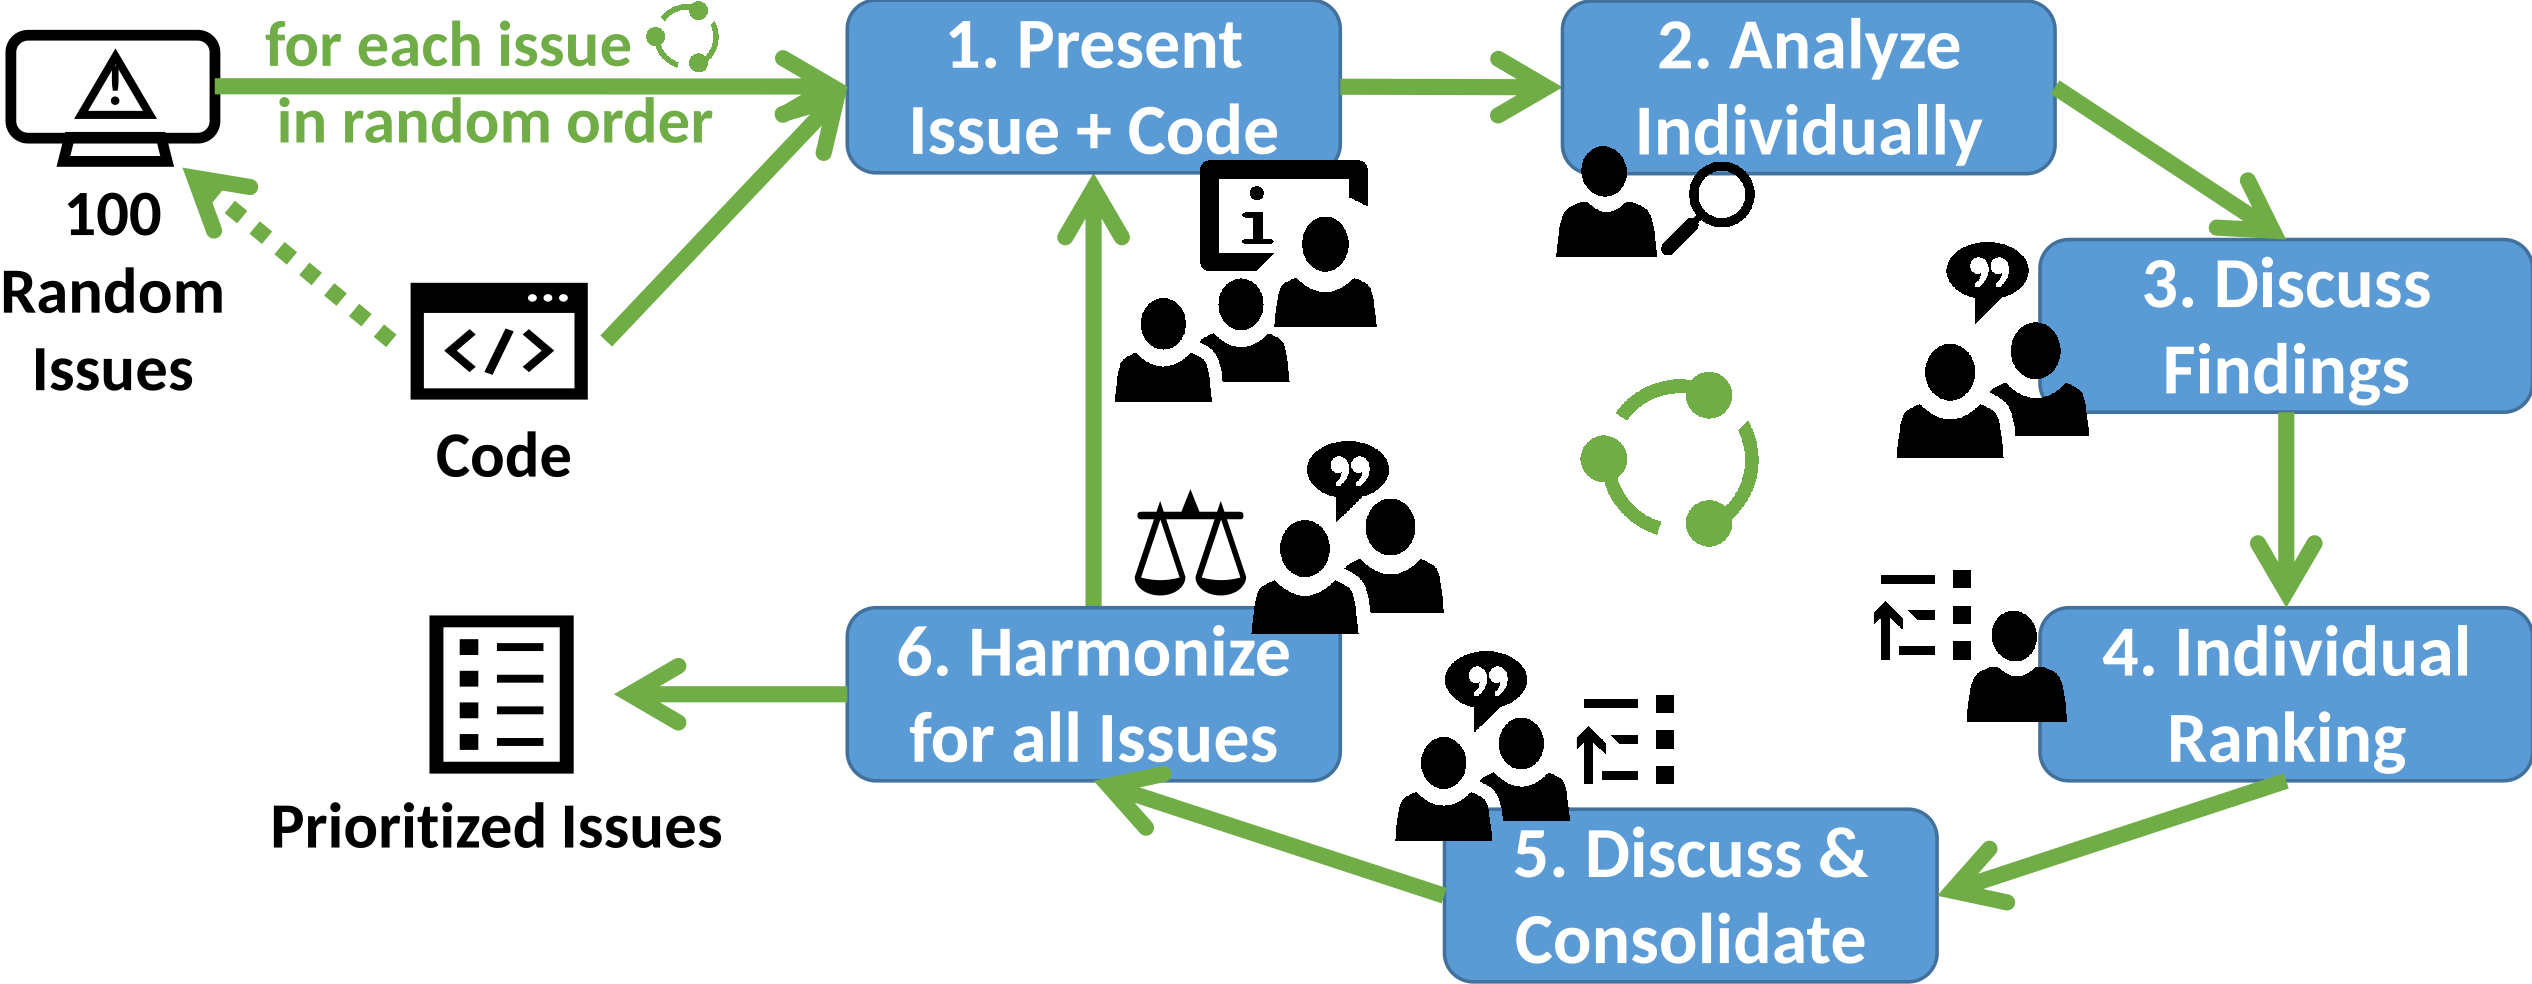
\includegraphics[width=.6\columnwidth]{figures/ManualPrio-KG.png}%width=0.8\textwidth
	\caption{Manual Issue Prioritization Workflow}
	\label{fig:ManualPrio}
\end{figure}

\subsubsection{Setup}
%We extracted randomly a set of 100 issues from the 6,284 ones calculated with SonarCube for iTrust and prioritized these manually before the results of the automated prioritization of the maximum flow analysis were known.
We randomly extracted two sets of 100 SonarQube issues each from iTrust's 6,284 issues and 159 issues calculated for the CWA. %the 159 for CWA.
We prioritized these manually before the results by applying \appr{} were known.
The rating was determined in group discussion sessions with four of the authors as illustrated in \autoref{fig:ManualPrio}.
Each issue was categorized from 1~(low) to 10~(high) %low to high %between 1 and 10
concerning its urgency to fix based on its security impact.
For that, its type and code location are taken into account in steps 2-5 in \autoref{fig:ManualPrio}:
\begin{enumerate}[label=\alph*), ref=\alph*)]
    \item What is the purpose of the code at the given location?
    \item What is the relevance for the project?
    \begin{enumerate}[label=\roman*), ref=\roman*)]
        \item Is it productive or test code?
        \item Is it a main functionality related to a requirement?
        \item What is the security relevance of the handled data?
        \item How accessible is the location from outside the system?
        \item How exploitable is the source code at the given location?
    \end{enumerate}
    \item Which security qualities (from the Quality Model) are addressed by the issue?
\end{enumerate}

\begin{figure}
    \centering
    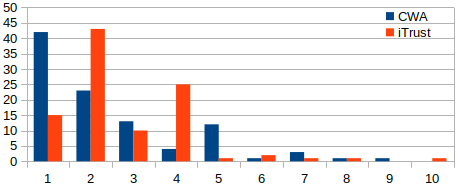
\includegraphics[width=.6\columnwidth]{figures/manual-rankings}
    \caption{Distribution of the manual issue priority categorizations for the two case studies.}
    \label{fig:manual-ranks}
\end{figure}

After a short discussion, full agreement was reached among all raters for each score.
In total, the rating took $\approx$120~min per project.
\autoref{fig:manual-ranks} shows how the 100 issues were ranked for the two case studies.
The majority of issues, 65 for CWA and 58 for iTrust, were rated with a priority of 2 or less. Only 6 issues for CWA and 5 for iTrust have a priority of 5 or higher, representing the group of most important issues for the projects.

%Trace dependencies are used by the tool to make up for the intuition about the code that the developer has, but the tool does not have.

The automated \appr\ prioritization technique does not use fixed priorities from 1 to 10, but assigns values based on the maximum flow reaching the issue.
SonarQube labels issues with five different severities ranging from \textit{Info} to \textit{Blocker} to which we assigned values from 0 to 4.
However, as the goal is to prioritize the findings, the absolute numbers are not relevant.
What we are interested in is the ordering. We compare the three rankings of the same 100 issues.

\subsubsection{Results}
%
In a first comparison, to study the general alignment of the prioritizations, we compared the prioritizations using the Spearman rank correlation coefficient\,\cite{10.2307/1412159}.
\autoref{tab:correlations} shows the %calculated
R-values and the significance level at which our results are significant.
These R-values indicate that all correlations are significant at a significance level of 0.01\,\cite{Whitlock2008ABD}.
The rankings calculated using \appr{} correlate much stronger with the manual rankings than SonarQube's severities.
In line with our basic assumption,  only very few issues ($\approx$4\%) are considered to be highly important for iTrust, in the manual and \appr 's ranking. In particular, only one issue is rated 10 manually, while there are very many critical issues according to SonarQube's severities---one fourth of all issues.
We made the same observation for the CWA.
Generally, \appr{} and the manual rankings agree upon issues being low, medium, or highly relevant.
E.g., for iTrust, the 40 lowest rated issues are the same in both orderings and besides one outlier all issues manually rated as important also got a high priority by \appr.
Yet, within these clusters of similar weights, the issues are shuffled. %negatively impacting the correlation.
This is not surprising, as the manual prioritization and SonarQube's severities are less fine-grained than \appr{} and an absolute order is hard to define.
These permutations are not necessarily faults, but have a negative impact on the correlation score, leading to generally low values.
In particular the ordering of issues of same priority is random.


\begin{table}
    \caption{Correlations of the automated prioritization and SonarQube's severities with the manually prioritized issues.}
    \label{tab:correlations}
    \centering
    \begin{tabular}{l|cc|c}
        \toprule
        & \multicolumn{2}{c|}{R-value} & Significance\\
        Project & \appr{} & SonarQube & Level \\
         \midrule
        iTrust & .4598 & .3023 & 0.01 \\
        CWA & .4709 & .3922 & 0.01 \\
         \bottomrule
    \end{tabular}
    \vspace{-14pt}
\end{table}

\begin{figure}
	\begin{center}
	\begin{subfigure}{.5\textwidth}
		\begin{center}
		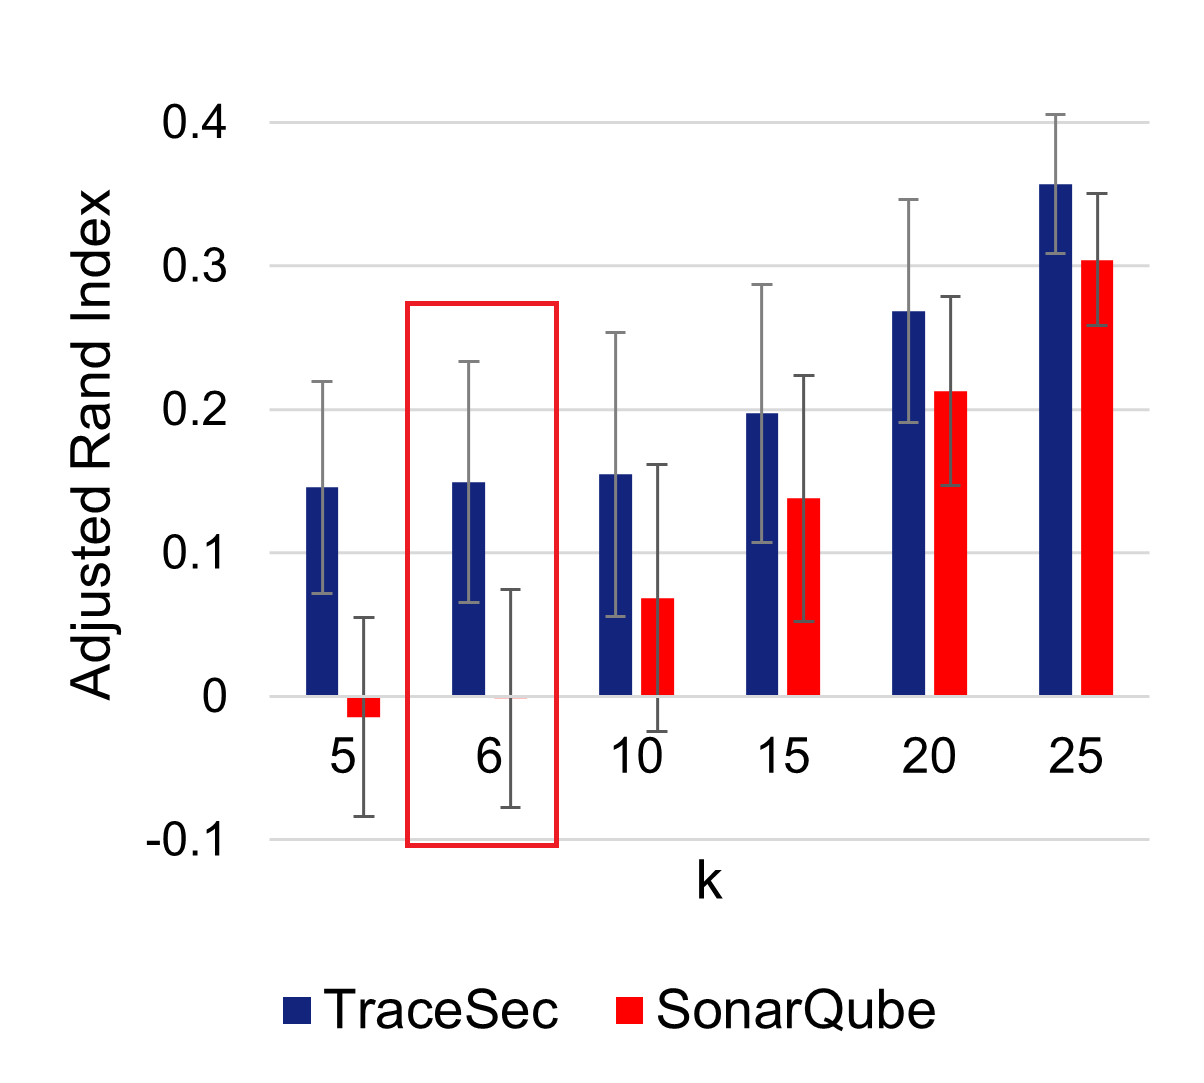
\includegraphics[width=.9\linewidth]{figures/topKiTrust}
		\caption{iTrust}
		\label{topKiTrust}
		\end{center}%
	\end{subfigure}%
	\begin{subfigure}{.5\textwidth}
		\begin{center}
		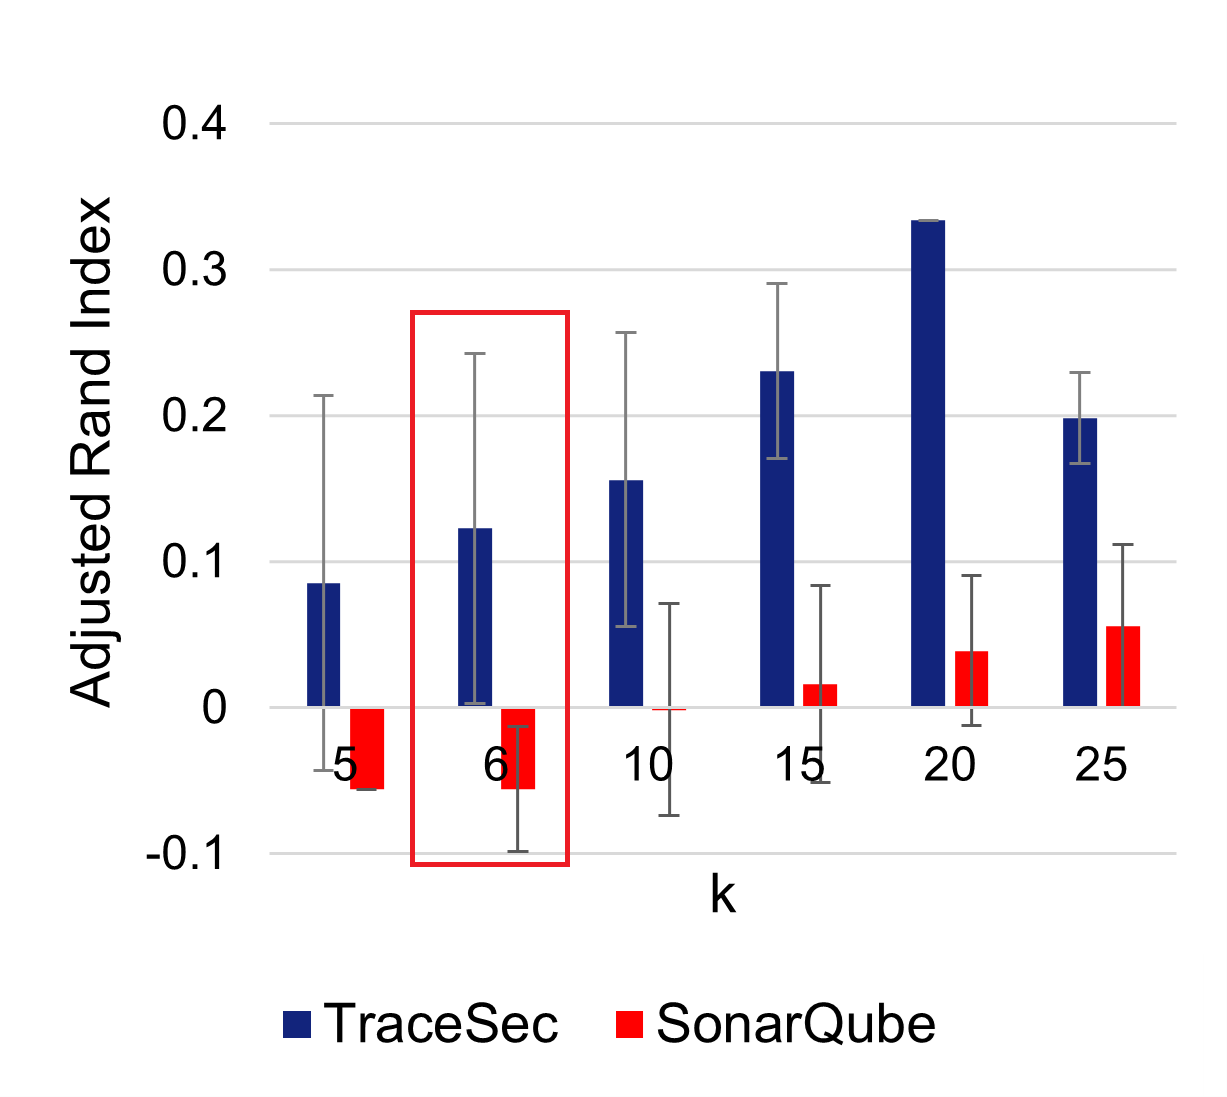
\includegraphics[width=.9\linewidth]{figures/topKcwa}%
		\caption{CWA}
		\label{topKCWA}
		\end{center}
	\end{subfigure}
	\caption{Adjusted Rand Index (ARI) for Partition of Top k Findings Compared to Manual Prioritization}
	\label{topK}
	\end{center}
\end{figure}

Thus, a more coarse grained comparison of the rankings based on clusters seems more appropriate.
In practice, developers are mainly interested in the most important issues to fix. To compare the two prioritizations in this regard, we checked %what percentage
the similarity
of the top k most important issues according to our manual prioritization %are also in
with
the top k most important issues according to the SonarQube rule priorities and \appr.
\autoref{topK} shows the Adjusted Rand Index~(ARI)\,\cite{Hubert1985,Santos2009} similarity of two-class partitions into top k and all other findings for k = 5 to 25.
The presented values are averages over 1,000 runs, where the issues with the same priority are randomly shuffled within that range.
These permutations make the evaluation robust against random effects of issues %sharing the same priority as others within the top-k group but
being cutoff from the top-k cluster due to ordering when there are more issues of the same priority than fit into the top-k.
The error-bars in \autoref{topK} indicate the respective standard deviation $\sigma$.
Here,  \appr\ clearly outperforms SonarQube.
The top 5, and for CWA also top 10, similarity of SonarQube is even lower than for a random partition.
%However, on CWA the similarity values are generally lower.
As can be seen in \autoref{fig:manual-ranks}, there are 6 issues for CWA that are labeled with a priority of 5 and higher, and 6 issues for iTrust that were manually labeled with a priority of 6 or higher.
Since all groups with lower priority labels become much larger, e.g., 12 additional issues for CWA with a priority of 4, we assume that these 6 issues are the most important issues for the two projects. %Accordingly, we choose k as 6 for the comparison.
%This choice of k also
Choosing k = 6
eliminates the possible randomness due to more issues being identically ranked than can be added to the top k group.
We highlight these values in \autoref{topK}.
The ARI similarity for the top 6 partition on iTrust is $0.15$ for \appr\ and $0.08$ for SonarQube.
On the CWA \appr\  achieves $0.12$ and SonarQube $-0.06$.
This matches the general pattern observed in \autoref{topK} and shows that \appr\ better reflects the priorities derived from project context as considered in the manual ranking.

As we do not have a real gold standard, the individual background of diverging ratings is relevant.
%Here we discuss some observations.
First, we observe that \appr{} does not distinguish issues within the test code from those in the actual system code.
In the manual rating, issues within the test code are treated more or less equally and generally rated to be of lower importance.
\appr{} reflects the dependencies of individual test cases to the main project and, thus, differentiates different cases.
Issues in test cases can cause falsely passed tests that do not test the intended behaviour.
We observed this in at least one case for iTrust.
Considering the importance of thorough testing in general and of security-critical functions specifically, to take this into account appears more plausible than the intuitive manual approach.

Issues with a low manual rating but medium priority in the flow analysis were  manually often considered false positives (of the static-analyzer tool) or irrelevant.
As stated above, our approach is not designed to detect false positives.
For that, the precision of the static analyzer itself would have to be increased, which is not the focus of this work.
Similarly, rules that are considered irrelevant, e.g., certain naming conventions, can be customized or deactivated.

In our dataset, we have a single outlier %issue #41
that is manually rated as rather important but has only low to medium importance concerning the flow analysis.
This particular issue resides in a field of a Java class that has only a few trace connections to the rest of the project.
Yet, it is accessible through the UI and, thus, exploitable.
Positively, this outlier still has in all three rankings a higher priority than other issues in the same class.
However, this shows potential for improvement, as fields are generally less connected with other artifacts than methods.
This needs to be addressed in parameter tuning in the configuration~file.%, which is examined in objective \ref{o2}.

%Considering the effort for the manual prioritization, already these results on the the small iTrust example with partially artificial re-engineerired artifacts and trace links with coarse granularity appear promising.


%iTrust is a small real world example.
%However, it is rather small and partially the artifacts and in particular the trace links are artificially re-engineered.
%The granularity of the traces is quite coarse grained.
%and size of sample (100) -> feasibility
%Discuss reliability of manual ranking vs. expected automated results / effort
%considering the manual effort for prioritization the result is close enough to help reduce work



\subsection{Adjustability}
To evaluate the adjustability to project-specific priorities~(\ref{o2}), we investigate the impact of weighting options as described in \autoref{edgeCap}.
While capacities of individual edge types can be adjusted through a configuration file using the presented DSL, as described in \autoref{DevArt}, the quality model is the most likely entry point for project-specific prioritization as this is where the stakeholder judgment is documented and applied.
The configuration file is only specified once by an expert and not edited during the usual development~process.

To evaluate the influence of these weighting instruments, we compare the results of the prioritization with different capacities for different quality aspects. %or edge types.

\subsubsection{Setup}
%We take again the 100 issues used for \ref{o1}.
%The priorities calculated in the effectiveness experiment serve as a reference.
We take again the 100 issues used for \ref{o1} and use the calculated priorities as a reference.
First, we investigate the impact of the priority values in the quality model by keeping the manual assignment of the priorities in the quality model %from the previous experiment
and multiplying these with different factors to get smaller and higher priorities.
In another run of the maximum flow analysis, we change the priorities in the quality model to assign a significantly higher priority to a single sub-tree of the quality model.
We compare the ordering analogously to the effectiveness evaluation \ref{o1}.

\subsubsection{Results}

\autoref{fig:weights} shows the correlations of the 100 issues prioritized using \appr{} with the prioritization from O1 for different capacities applied to a four-level ranking in the quality model.
The applied capacities are shown on the x-axis and are ordered increasingly.
The capacities used in O1 are 25-50-75-100.
Accordingly, this prioritization is identical with the one of O1, which corresponds with an R-value of 1.
Increasing the priorities further has no impact on the prioritization; with the capacities used in O1, the bottleneck of the flow network (known as \emph{minimum cut}\,\cite{1056816,ford_fulkerson_1956}) %(described as minimum cut in literature\,\cite{1056816,ford_fulkerson_1956})
is not in the quality model.
On the other hand, the lower capacities in the quality model lead to increasing differences in the prioritizations for iTrust, which is reflected by a lower R-value.
For the CWA, only capacities 1-2-3-4 lead to a slight difference with a correlation of .9999 instead of 1.
However, the correlation with the manual ranking improved slightly to .4711, indicating that the minimum cut has been moved into the quality model.
Unfortunately, as we only support natural numbers, reducing the weights further is not possible. Here, we suffer from the fact that the CWA only has a very abstract component diagram which allows few trace links that limit the capacity that can be propagated from the quality model towards the issues.

\begin{figure}
    \centering
    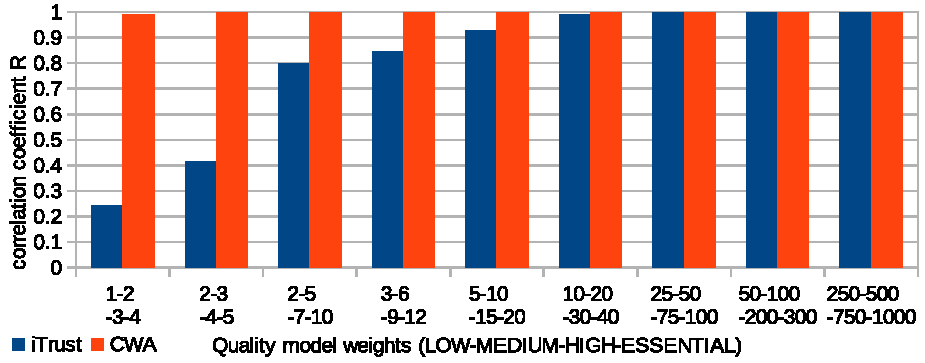
\includegraphics[width=.75\columnwidth]{figures/impact-qm-weights.pdf}
    \caption{Impact of the Priority Values in the Quality Model}
    %\caption{Impact of the Weight Values in the Quality Model on the Prioritization}
    \label{fig:weights}
\end{figure}

Altogether, choosing good capacities (representing the priorities in the quality model) is essential for a prioritization that reflects the importance of qualities.
If the capacity is chosen too low, the minimum cut through the network is located in the quality model and the other artifacts might have no impact on the prioritization.
If the capacities are chosen too high, the issues are only prioritized based on the other artifacts.
A suitable trade-off has to be found.
Whether the priorities in the quality model can influence the prioritization at all is discussed based on the second part of this evaluation~objective.

%\begin{figure}
%    \centering
%    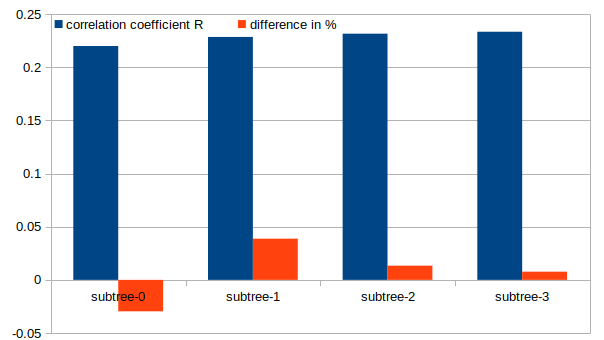
\includegraphics[width=\columnwidth]{figures/impact-qm-trees.png}
%    \caption{Impact of the prioritization of a single sub-tree of the quality model on the prioritization}
%    \label{fig:trees}
%\end{figure}

\autoref{tab:trees} shows the correlations of the prioritization from O1 with the prioritizations calculated when assigning high importance to only one of the sub-trees of iTrust's quality model and among each other.
With R-values close to 1 the
%single
prioritizations are very similar but still, the changes in the quality model show an effect on the prioritization.
As we already observed that the parts of the flow network representing the other artifacts played a central role in the prioritization, these results are not unexpected.
Still, it shows that already with a small and highly interconnected quality model users can influence the~prioritization.

For the CWA we got identical prioritizations (a correlation of~1) regardless of which tree was set to high importance.
As the highest ranked issue of the CWA only got a rating of 23, this is not surprising as in this experiment the lowest priority in the quality model reflects a capacity of 25.
As in the first part of this experiment, there are too few trace links between the quality model and the architecture.

\begin{table}
    \centering
    \caption{Correlation Matrix Showing the Impact of the Prioritization of a Single Sub-tree of iTrust's Quality Model}
    \label{tab:trees}
%    \footnotesize
    \begin{tabular}{r|rrrr}
        \toprule
         & tree 1 & tree 2 & tree 3 & tree 4  \\
         \midrule
        O1 & .9898 & .9919 & .9950 & .9897 \\
        tree 1 & & .9966 &	.9931 & .9997 \\
        tree 2 & & & .9965 &	.9969 \\
        tree 3 & & & & .9934 \\
        \bottomrule
    \end{tabular}
\end{table}


Overall, the influence of the quality model on prioritization is lower than expected.
The exemplary quality models are rather small and highly interconnected as they only contain essential security-related aspects.
Especially the CWA shows that a sufficient amount of trace links from the quality model to the other artifacts is necessary to allow adjustability.
We expect more influence for not reverse-engineered models with more project context.

%\subsection{Robustness}
%
%	Creating trace links is expensive and error prone and in practice imperfect trace links are likely.
%	Besides this, particularly design models such as UML models are often rather less used in practice\,\cite{Gorschek2014} and if present are probably not of the highest quality.
%	Therefore, we are interested in how well TraceSEC performs in presence of imperfect trace links and planning artifacts (\ref{o4}).
%	The overall question is whether lesser organized projects can still benefit from \appr{}.
%	To understand the quality requirements on needed artifacts such as models and trace links, we are going to investigate how the accuracy of traceability links, i.e., connections within models and trace links between models and code, affect the importance rankings.
%
%\subsubsection{Setup}
%	To estimate the impact of imperfect traceability, we need to consider two types of trace links separately.
%	First, internal links within artifacts (requirements \& design models), and second, external links between different artifacts (QM → requirements → design → code).
%	The former indicates the quality of the artifacts produced, while the latter indicates how well trace links between different artifacts are created and maintained.
%	Therefore, we considered these two types of trace links independently.
%
%
%
%	To evaluate how robust TraceSEC is to imperfect trace links, we injected faults into the trace links by randomly deleting existing trace links or randomly creating additional trace links.
%	Additions and deletions were performed independently, and we iteratively added and deleted between 0\% and 50\% of all trace links.
%	After each change, we measured the quality of the prioritization in terms of correlation with the manual baseline.
%	Since only detailed requirements and design models are available for iTrust, we performed this experiment only on this case study.
%
%
%
%\subsubsection{Results}
%%
%	In  \autoref{tab:robustness} we show how much the correlation with the manual base line changed for the addition of false positives (fp) and deletions leading to false negatives (fn).
%	When looking at the outcomes, missing external trace links severely impact the prioritization. However, false positives do not seem to be a  problem (it is often better to have a wrong trace link instead of no trace link).
%	Therefore, external trace links must not be precise and internal trace links can make up for not accurate external trace links.
%	On their own, internal trace links have only a low impact.
%	Since the used models of iTrust were reverse engineered from the code and therefore only few information is added, this could be an explanation for this observed low impact but therefore high robustness.
%	However, there is still a slight negative impact.
%
%\begin{figure}
%
%	\begin{subfigure}{\textwidth}
%		\footnotesize
%		\setlength{\tabcolsep}{2pt}
%		\centering
%		\begin{tabularx}{\textwidth}{>{\bfseries}r|XXXXXXXXXXXXXXXX}
%			fp\textbackslash fn &	\textbf{0.0\%} &	\textbf{0.1\%} &	\textbf{0.2\%} &	\textbf{0.5\%} &	\textbf{1.0\%} &	\textbf{2.0\%} &	\textbf{5.0\%} &	\textbf{10.0\%} &	\textbf{15.0\%} &	\textbf{20.0\%} &	\textbf{25.0\%} &	\textbf{30.0\%} &	\textbf{35.0\%} &	\textbf{40.0\%} &	\textbf{45.0\%} &	\textbf{50.0\%} \\
%			\hline
%			0.0\%   &	0.00\% &	\rcolor{0.00} &	\rcolor{0.00} & \rcolor{0.00} & \rcolor{-0.35} &	\rcolor{-0.36} & \rcolor{-1.49} & \rcolor{-4.21} & \rcolor{-6.43} & \rcolor{-6.43} & \rcolor{-6.53} & \rcolor{-7.36} & \rcolor{-7.70} & \rcolor{-8.59} & \rcolor{-9.94} & \rcolor{-12.09} \\
%			0.1\%   &	\rcolor{1.29} & \rcolor{1.23} & \rcolor{1.23} & \rcolor{0.99} & \rcolor{0.73} & \rcolor{0.41} & \rcolor{-0.72} & \rcolor{-2.02} & \rcolor{-2.28} & \rcolor{-2.48} & \rcolor{-3.65} & \rcolor{-2.81} & \rcolor{-4.21} & \rcolor{-3.32} & \rcolor{-3.09} & \rcolor{-5.35} \\
%			0.2\%   &	\rcolor{2.06} & \rcolor{2.01} & \rcolor{2.04} & \rcolor{2.02} & \rcolor{2.01} & \rcolor{2.39} & \rcolor{0.28} & \rcolor{-1.55} & \rcolor{-1.84} & \rcolor{-1.71} & \rcolor{-2.01} & \rcolor{-1.65} & \rcolor{-3.01} & \rcolor{-2.84} & \rcolor{-3.22} & \rcolor{-2.76} \\
%			0.5\%   &	\rcolor{2.25} & \rcolor{2.17} & \rcolor{2.17} & \rcolor{2.17} & \rcolor{2.17} & \rcolor{2.17} & \rcolor{1.73} & \rcolor{0.24} & \rcolor{-1.03} & \rcolor{-0.73} & \rcolor{-1.86} & \rcolor{-2.88} & \rcolor{-2.93} & \rcolor{-3.29} & \rcolor{-4.67} & \rcolor{-4.93} \\
%			1.0\%   &	\rcolor{2.25} & \rcolor{2.17} & \rcolor{2.17} & \rcolor{2.17} & \rcolor{2.17} & \rcolor{2.25} & \rcolor{1.59} & \rcolor{0.92} & \rcolor{0.72} & \rcolor{0.22} & \rcolor{0.28} & \rcolor{0.08} & \rcolor{-1.36} & \rcolor{-1.45} & \rcolor{-1.56} & \rcolor{-1.17} \\
%			2.0\%   &	\rcolor{2.25} & \rcolor{2.17} & \rcolor{2.16} & \rcolor{2.16} & \rcolor{2.16} & \rcolor{1.63} & \rcolor{1.58} & \rcolor{1.65} & \rcolor{0.60} & \rcolor{-1.61} & \rcolor{-1.59} & \rcolor{-0.88} & \rcolor{-0.77} & \rcolor{-0.91} & \rcolor{-0.81} & \rcolor{-0.80} \\
%			5.0\%   &	\rcolor{2.43} & \rcolor{2.35} & \rcolor{2.35} & \rcolor{2.35} & \rcolor{2.35} & \rcolor{2.35} & \rcolor{2.25} & \rcolor{1.99} & \rcolor{0.50} & \rcolor{0.55} & \rcolor{0.18} & \rcolor{-0.37} & \rcolor{0.01} & \rcolor{-0.64} & \rcolor{-0.59} & \rcolor{-0.62} \\
%			10.0\%  &	\rcolor{2.42} & \rcolor{2.33} & \rcolor{2.33} & \rcolor{2.33} & \rcolor{2.33} & \rcolor{2.18} & \rcolor{2.21} & \rcolor{2.60} & \rcolor{2.32} & \rcolor{2.01} & \rcolor{2.15} & \rcolor{1.57} & \rcolor{1.33} & \rcolor{1.17} & \rcolor{1.14} & \rcolor{1.13} \\
%			15.0\%  &	\rcolor{2.42} & \rcolor{2.33} & \rcolor{2.33} & \rcolor{2.33} & \rcolor{2.33} & \rcolor{2.33} & \rcolor{2.33} & \rcolor{1.68} & \rcolor{1.24} & \rcolor{1.23} & \rcolor{1.10} & \rcolor{1.03} & \rcolor{1.03} & \rcolor{0.91} & \rcolor{0.91} & \rcolor{0.92} \\
%			20.0\%  &	\rcolor{2.42} & \rcolor{2.33} & \rcolor{2.33} & \rcolor{2.33} & \rcolor{2.33} & \rcolor{2.33} & \rcolor{2.33} & \rcolor{1.97} & \rcolor{1.97} & \rcolor{1.97} & \rcolor{1.97} & \rcolor{2.11} & \rcolor{1.79} & \rcolor{1.54} & \rcolor{1.54} & \rcolor{1.54} \\
%			25.0\%  &	\rcolor{2.42} & \rcolor{2.33} & \rcolor{2.33} & \rcolor{2.33} & \rcolor{2.33} & \rcolor{2.33} & \rcolor{2.17} & \rcolor{2.17} & \rcolor{2.42} & \rcolor{1.81} & \rcolor{1.81} & \rcolor{1.90} & \rcolor{1.90} & \rcolor{1.95} & \rcolor{1.95} & \rcolor{1.95} \\
%			30.0\%  &	\rcolor{2.42} & \rcolor{2.33} & \rcolor{2.33} & \rcolor{2.33} & \rcolor{2.33} & \rcolor{2.33} & \rcolor{2.33} & \rcolor{2.30} & \rcolor{2.30} & \rcolor{2.18} & \rcolor{2.30} & \rcolor{2.44} & \rcolor{2.19} & \rcolor{2.17} & \rcolor{2.17} & \rcolor{2.17} \\
%			35.0\%  &	\rcolor{2.42} & \rcolor{2.33} & \rcolor{2.33} & \rcolor{2.33} & \rcolor{2.33} & \rcolor{2.33} & \rcolor{2.33} & \rcolor{2.33} & \rcolor{2.07} & \rcolor{1.97} & \rcolor{1.97} & \rcolor{2.07} & \rcolor{2.07} & \rcolor{2.07} & \rcolor{2.07} & \rcolor{2.07} \\
%			40.0\%  &	\rcolor{2.42} & \rcolor{2.33} & \rcolor{2.33} & \rcolor{2.33} & \rcolor{2.33} & \rcolor{2.33} & \rcolor{2.33} & \rcolor{2.30} & \rcolor{2.30} & \rcolor{2.18} & \rcolor{2.18} & \rcolor{2.42} & \rcolor{2.42} & \rcolor{2.41} & \rcolor{2.41} & \rcolor{2.41} \\
%			45.0\%  &	\rcolor{2.42} & \rcolor{2.33} & \rcolor{2.33} & \rcolor{2.33} & \rcolor{2.33} & \rcolor{2.33} & \rcolor{2.33} & \rcolor{2.33} & \rcolor{2.33} & \rcolor{2.21} & \rcolor{2.21} & \rcolor{2.33} & \rcolor{2.33} & \rcolor{2.33} & \rcolor{2.33} & \rcolor{2.33} \\
%			50.0\%  &	\rcolor{2.42} & \rcolor{2.33} & \rcolor{2.33} & \rcolor{2.33} & \rcolor{2.33} & \rcolor{2.33} & \rcolor{2.33} & \rcolor{2.33} & \rcolor{2.33} & \rcolor{2.21} & \rcolor{1.92} & \rcolor{1.92} & \rcolor{1.92} & \rcolor{1.73} & \rcolor{1.73} & \rcolor{1.73} \\
%		\end{tabularx}
%
%		\caption{Changes for external trace links between different artifacts.}
%	\end{subfigure}
%
%	\begin{subfigure}{\textwidth}
%		\footnotesize
%		\setlength{\tabcolsep}{2pt}
%		\centering
%		\begin{tabularx}{\textwidth}{>{\bfseries}r|XXXXXXXXXXXXXXXX}
%			fp\textbackslash fn &	\textbf{0.0\%} &	\textbf{0.1\%} &	\textbf{0.2\%} &	\textbf{0.5\%} &	\textbf{1.0\%} &	\textbf{2.0\%} &	\textbf{5.0\%} &	\textbf{10.0\%} &	\textbf{15.0\%} &	\textbf{20.0\%} &	\textbf{25.0\%} &	\textbf{30.0\%} &	\textbf{35.0\%} &	\textbf{40.0\%} &	\textbf{45.0\%} &	\textbf{50.0\%} \\
%			\hline
%			0.0\% & 0.00\% & \rcolor{0.00} & \rcolor{0.00} & \rcolor{0.00} & \rcolor{0.00} & \rcolor{0.00} & \rcolor{0.02} & \rcolor{0.06} & \rcolor{0.06} & \rcolor{0.02} & \rcolor{0.03} & \rcolor{0.03} & \rcolor{0.00} & \rcolor{0.02} & \rcolor{0.07} & \rcolor{0.09} \\
%			0.1\% & \rcolor{-0.01} & \rcolor{-0.01} & \rcolor{-0.01} & \rcolor{-0.01} & \rcolor{-0.01} & \rcolor{-0.01} & \rcolor{-0.01} & \rcolor{0.00} & \rcolor{-0.05} & \rcolor{-0.04} & \rcolor{-0.08} & \rcolor{-0.08} & \rcolor{-0.07} & \rcolor{-0.01} & \rcolor{0.04} & \rcolor{0.03} \\
%			0.2\% & \rcolor{0.00} & \rcolor{0.00} & \rcolor{0.00} & \rcolor{0.02} & \rcolor{0.01} & \rcolor{0.01} & \rcolor{-0.03} & \rcolor{-0.04} & \rcolor{-0.02} & \rcolor{-0.03} & \rcolor{-0.03} & \rcolor{-0.03} & \rcolor{-0.03} & \rcolor{-0.06} & \rcolor{-0.06} & \rcolor{-0.06} \\
%			0.5\% & \rcolor{0.00} & \rcolor{0.00} & \rcolor{-0.01} & \rcolor{-0.01} & \rcolor{-0.01} & \rcolor{-0.01} & \rcolor{-0.01} & \rcolor{0.00} & \rcolor{0.03} & \rcolor{0.05} & \rcolor{0.05} & \rcolor{0.05} & \rcolor{0.02} & \rcolor{-0.01} & \rcolor{-0.01} & \rcolor{-0.01} \\
%			1.0\% & \rcolor{-0.01} & \rcolor{-0.01} & \rcolor{-0.01} & \rcolor{-0.01} & \rcolor{-0.01} & \rcolor{-0.01} & \rcolor{-0.01} & \rcolor{-0.02} & \rcolor{0.02} & \rcolor{0.02} & \rcolor{0.01} & \rcolor{0.01} & \rcolor{0.01} & \rcolor{0.01} & \rcolor{0.01} & \rcolor{0.01} \\
%			2.0\% & \rcolor{-0.02} & \rcolor{-0.02} & \rcolor{-0.01} & \rcolor{-0.01} & \rcolor{-0.01} & \rcolor{-0.01} & \rcolor{-0.01} & \rcolor{-0.02} & \rcolor{-0.01} & \rcolor{-0.01} & \rcolor{0.03} & \rcolor{0.03} & \rcolor{0.03} & \rcolor{0.03} & \rcolor{0.03} & \rcolor{0.02} \\
%			5.0\% & \rcolor{-0.02} & \rcolor{-0.02} & \rcolor{-0.02} & \rcolor{-0.02} & \rcolor{-0.02} & \rcolor{-0.01} & \rcolor{-0.01} & \rcolor{-0.02} & \rcolor{0.06} & \rcolor{0.06} & \rcolor{0.06} & \rcolor{0.06} & \rcolor{0.05} & \rcolor{0.05} & \rcolor{0.05} & \rcolor{0.05} \\
%			10.0\% & \rcolor{-0.06} & \rcolor{-0.06} & \rcolor{-0.06} & \rcolor{-0.06} & \rcolor{-0.06} & \rcolor{-0.06} & \rcolor{-0.06} & \rcolor{-0.07} & \rcolor{-0.07} & \rcolor{-0.07} & \rcolor{-0.07} & \rcolor{-0.07} & \rcolor{-0.06} & \rcolor{-0.06} & \rcolor{-0.06} & \rcolor{-0.06} \\
%			15.0\% & \rcolor{-0.06} & \rcolor{-0.06} & \rcolor{-0.06} & \rcolor{-0.06} & \rcolor{-0.06} & \rcolor{-0.06} & \rcolor{-0.06} & \rcolor{-0.06} & \rcolor{-0.07} & \rcolor{-0.07} & \rcolor{-0.06} & \rcolor{-0.03} & \rcolor{0.18} & \rcolor{0.18} & \rcolor{0.18} & \rcolor{0.18} \\
%			20.0\% & \rcolor{-0.06} & \rcolor{-0.06} & \rcolor{-0.06} & \rcolor{-0.06} & \rcolor{-0.06} & \rcolor{-0.06} & \rcolor{-0.06} & \rcolor{-0.06} & \rcolor{-0.07} & \rcolor{-0.07} & \rcolor{-0.07} & \rcolor{-0.07} & \rcolor{-0.04} & \rcolor{-0.04} & \rcolor{-0.04} & \rcolor{-0.04} \\
%			25.0\% & \rcolor{-0.06} & \rcolor{-0.06} & \rcolor{-0.06} & \rcolor{-0.06} & \rcolor{-0.06} & \rcolor{-0.06} & \rcolor{-0.06} & \rcolor{-0.10} & \rcolor{-0.10} & \rcolor{-0.10} & \rcolor{-0.11} & \rcolor{-0.11} & \rcolor{-0.14} & \rcolor{-0.14} & \rcolor{-0.09} & \rcolor{-0.09} \\
%			30.0\% & \rcolor{-0.06} & \rcolor{-0.06} & \rcolor{-0.06} & \rcolor{-0.06} & \rcolor{-0.06} & \rcolor{-0.06} & \rcolor{-0.06} & \rcolor{-0.06} & \rcolor{-0.05} & \rcolor{-0.05} & \rcolor{-0.05} & \rcolor{-0.05} & \rcolor{-0.05} & \rcolor{-0.05} & \rcolor{-0.05} & \rcolor{-0.05} \\
%			35.0\% & \rcolor{-0.06} & \rcolor{-0.06} & \rcolor{-0.06} & \rcolor{-0.06} & \rcolor{-0.06} & \rcolor{-0.06} & \rcolor{-0.06} & \rcolor{-0.06} & \rcolor{-0.06} & \rcolor{-0.06} & \rcolor{-0.06} & \rcolor{-0.06} & \rcolor{-0.06} & \rcolor{-0.06} & \rcolor{-0.06} & \rcolor{-0.06} \\
%			40.0\% & \rcolor{-0.06} & \rcolor{-0.06} & \rcolor{-0.06} & \rcolor{-0.06} & \rcolor{-0.06} & \rcolor{-0.06} & \rcolor{-0.06} & \rcolor{-0.06} & \rcolor{-0.06} & \rcolor{-0.06} & \rcolor{-0.06} & \rcolor{-0.06} & \rcolor{-0.06} & \rcolor{-0.06} & \rcolor{-0.06} & \rcolor{-0.06} \\
%			45.0\% & \rcolor{-0.06} & \rcolor{-0.06} & \rcolor{-0.06} & \rcolor{-0.06} & \rcolor{-0.06} & \rcolor{-0.06} & \rcolor{-0.06} & \rcolor{-0.06} & \rcolor{-0.06} & \rcolor{-0.06} & \rcolor{-0.06} & \rcolor{-0.06} & \rcolor{-0.06} & \rcolor{-0.06} & \rcolor{-0.06} & \rcolor{-0.06} \\
%			50.0\% & \rcolor{-0.06} & \rcolor{-0.06} & \rcolor{-0.06} & \rcolor{-0.06} & \rcolor{-0.06} & \rcolor{-0.06} & \rcolor{-0.06} & \rcolor{-0.06} & \rcolor{-0.07} & \rcolor{-0.07} & \rcolor{-0.07} & \rcolor{-0.07} & \rcolor{-0.07} & \rcolor{-0.07} & \rcolor{-0.07} & \rcolor{-0.07} \\
%		\end{tabularx}
%		\caption{Changes for internal trace links within requirements and design models.}
%	\end{subfigure}
%
%	\small
%	\setlength{\tabcolsep}{2pt}
%	\begin{tabular}{|c|c|c|c|c|c|c|c|c|c|c|c|c|}
%		\cellcolor{Red} < -10\% &
%		\cellcolor{Red!75} < -8\% &
%		\cellcolor{BurntOrange!75} < -6\% &
%		\cellcolor{YellowOrange!75} < -4\% &
%		\cellcolor{Goldenrod!85} < -2\% &
%		\cellcolor{Yellow!85} < -1\% &
%		\cellcolor{Yellow!40} -1\% < \& < 1\% &
%		\cellcolor{ForestGreen!17} > 1\% &
%		\cellcolor{ForestGreen!33} > 2\% &
%		\cellcolor{ForestGreen!50} > 4\% &
%		\cellcolor{ForestGreen!67} > 6\% &
%		\cellcolor{OliveGreen!70} > 8\% &
%		\cellcolor{OliveGreen!100} > 10\%\\
%	\end{tabular}
%
%	\caption{Average change in correlation with the manual baseline after adding (fp) or deleting (fn) trace links.}
%	\label{tab:robustness}
%\end{figure}
%
%\begin{figure}
%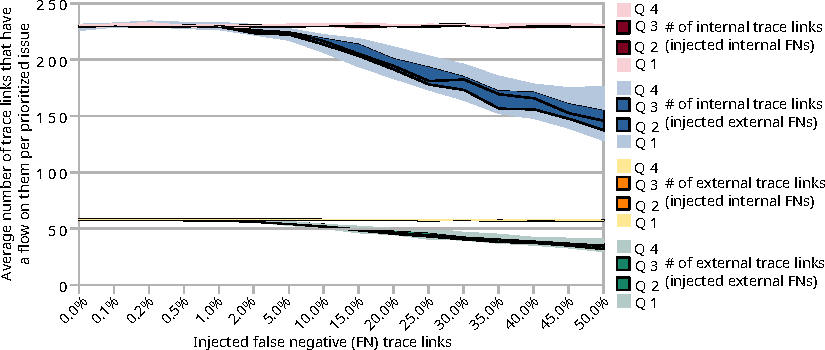
\includegraphics[width=.7\columnwidth]{figures/fns-edges.pdf}
%\caption{Number of internal and external trace links used for prioritization dependent on the number of false negative trace links}
%\label{fig:fnsEdges}
%\end{figure}
%
%
%	To better understand the results, we measured for the cases in which we only injected false negatives (FNs), i.e., deleting external or internal trace links how many of the edges in the flow network corresponding to them carry a flow when prioritizing an issue and how much flow this is per edge.
%	As visible in \autoref{fig:fnsEdges}, the number of as well internal as external trace links that have a flow on them decreases with the number of deleted external trace links (FNs).
%	Thereby, the number of internal trace links decreases stronger than the number of external trace links.
%	If internal trace links are deleted, the numbers stay consistent.
%	This fits to the results shown in \autoref{tab:robustness}, in which we also do not see a change for deleted internal trace links.
%	Since as well the number of external trace links as internal trace links over which a flow is propagated decreases with increasing FNs, this implies that combinations of previously unused internal trace links cannot compensate missing external trace links to a notable extend.
%	Instead, with deleted external trace links entire sub-graphs become uncreachable.
%	When measuring the average flow across each trace link, we observed the same behavior as the number of trace links, implying also that the utilization of the used trace links, i.e., propagating additional flow over previously not saturated trace links, does not increase.
%
%
%\begin{figure}
%	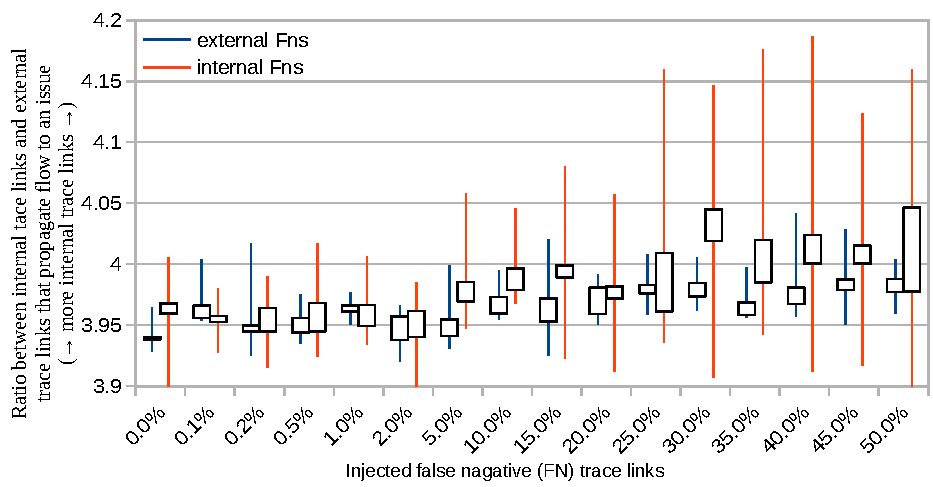
\includegraphics[width=.6\columnwidth]{figures/ratio-internal-to-external-tracelinks.pdf}
%	\caption{Number of internal trace links to external trace links dependent on the number of false negative trace links}
%	\label{fig:intVsExt}
%\end{figure}
%
%	When comparing the usage of external and internal trace links in the prioritization, meaning over which of them flow is propagated, we notice that the higher the number of false negative trace links gets, the more internal trace links are involved in the prioritization of an issue (see \autoref{fig:intVsExt}).
%	While this trend can be observed to some extent for both, false negative internal trace links and external trace links, it is more pronounced for deleted external trace links.
%	This indicates that internal trace links, e.g., design models or derived from code, play an essential role in distributing importance allowing for external trace links not immediately pointing to concrete issue locations, and allow the prioritization to also function to some extent for missing external trace links.
%
%
%Overall, this experiment indicates that even low quality design models and imperfect trace links are sufficient for gaining benefit from TraceSEC.
%Considering alternatives such as the SonarQube rule priorities for prioritizing issues, even in the worst case in which 50\% of all trace links have been deleted (a 12.09\% lower correlation coefficient), the prioritization of TraceSec still correlates stronger with the manual base line than the prioritization based on rule priorities (a correlation coefficient of .4041 for TraceSEC, while, according to \autoref{tab:correlations}, SonarQube rule priorities resulted only in .3023).
%Therefore, we can conclude that it is likely that even lesser organized projects can benefit from TraceSEC.
%Our deeper investigation of how internal and external trace links behave in this experiment suggests that it may be more beneficial to optimize external trace links than internal trace links.
%However, since the two go hand in hand, artifacts containing internal trace links, such as requirements or design models, could be a means of optimizing external trace links between them.


\subsection{Performance}
%
	Although often not explicitly measured, the continuous manual prioritization of issues adds significant overhead to the development of secure software systems.
	When only prioritizing issues and not interweaving this task with other development activities, the time we needed for prioritizing the issues of our baseline gives an indication of the involved overhead.
	Including discussions, the prioritization of 100 issues took us 120 minutes.
	Although, a single developer familiar with the project will be faster, significant overhead is still added.
	To this end, the automated prioritization of \appr{} aims at providing faster issue prioritization.
	To assess the benefit of \appr{}~(\ref{o3}), we have to consider two cost factors.
	First, unlike the manual prioritization \appr{} has an overhead for setting up the tooling.
	The second factor is the actual time needed for prioritization.




	\textit{1) Setup:}
	As discussed above, setting up \appr{} comes usually with relatively low cost since it works out of the box for most kinds of models.
	Custom models can be added to \appr{} by writing a few lines of configuration files.
	However, fine-tuning parameters, if needed, can be a significant effort but must not be invested upfront but we expect some continuous effort.
	Unfortunately, we have no practical experiences on this effort yet.
	For our own experiments, we needed less than 15 minutes to set up \appr{}, which included writing the needed configurations.


	\textit{2) Execution:}
	Wile the setup adds a static overhead, the actual execution of \appr{} takes time each time it is executed.
	Also, the time needed depends on the size of the flow network to create and analyze, i.e., the size of the project for which issues should be prioritized.
	Excluding the flow network construction, prioritizing 100 issues of iTrust (~70k LLOC) takes 23.9 seconds on average with TraceSEC.
	Since, the literature has extensively discussed the scalability of solving the max-flow problem and developed efficient algorithms\,\cite{ford_fulkerson_1956,dinic1970algorithm}, we expect no issues for larger projects.
To this end, for \ref{o3}, it remains to evaluate the scalability of the flow network~construction to determine the the performance gain of \appr{} compared to the manual prioritization.

\subsubsection{Setup}
%
To evaluate the scalability of constructing  flow networks, we measure the construction time for input data representing different-sized software projects. While plenty of real-world open-source Java projects exist that could be used, usually, requirements, design models, and trace links among them are not publicly available. For this reason, we randomly generated quality models, requirements models, component diagrams, and program models representing software projects of different sizes.

We have to ensure at model construction that the relation of nodes and references among these nodes corresponds with these of real-world projects.
Thus, we start with generating program models whose node and reference distributions correspond to those of 20 program models created in other works from real-world projects of different sizes (ranging from 1,197 to 201,541 logical lines of code)\,\cite{peldszus2016continuous,Peldszus2022}.
Afterward, we clustered the types contained in the program model for creating a UML component diagram as well as trace links.
Thereby, each cluster of types is linked to a component in the requirements diagram and the relations among the types are aggregated to inter component connections.
For each of these components, we generated two to four requirements and arranged these in the requirements model according to the relations observed in iTrust's requirements model.
Finally, we randomly generated a quality model whose size correlates with the number of requirements and randomly added trace links to these.
This way, we achieve input data whose relation among nodes and edges and also the relation among the sizes of the different models is realistic.
Furthermore, as we know the sizes of program models for software projects of different sizes from literature\,\cite{peldszus2016continuous}, we can state to which project size in terms of lines of code the generated models relate.

Using this generation approach, we generated random input data of different sizes with realistic distributions of nodes, relations, and trace links for which we measured the time required to construct the flow network.
We generated input data corresponding to projects between sizes of
%200,000 and 4,000,000
200k and 4x10$^6$
logical lines of code (LLOC) in steps of 100k %100,000
LLOC. For every size, we generated 10 different samples and report the average values.

\subsubsection{Results}
%
\autoref{fig:scaleability} shows the execution times of the flow network construction for input data representing software projects of different sizes.
As expected, the measured time increases with the input data size.
For medium-sized projects (below one million lines of code), we stay below two minutes that allows issue prioritization during development in an IDE.
For larger projects with up to three million lines of code, creation is possible on a consumer notebook (Intel i7-1165G7, 32GB RAM) in below one~hour.

\begin{figure}
    \centering
    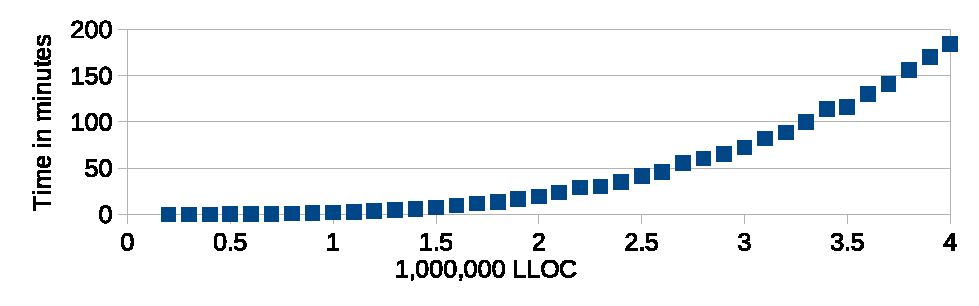
\includegraphics[width=.65\columnwidth]{figures/tracesec-scalability.eps}
    \caption{Scalability of the Flow Network Construction}
    \label{fig:scaleability}
\end{figure}

The scalability of the current implementation suffers from exponential time requirements when adding new elements to the base models (quality model, requirements, etc.) because the trace model has to be built anew with each change.
In future work, the prioritization could be calculated based on model deltas on a continuous integration server, which could then present the prioritized issues.

	Overall, it is likely that even a single execution of \appr{} saves enough time compared to manual prioritization to make up for the setup overhead.
	Assuming that \appr{} is executed with every nightly build, this allows for continuous prioritization of detected issues while saving significant time usually spent for manual prioritization.
	Even if some additional time is spent to optimize the configuration of \appr{}, e.g., monthly or quarterly taking two hours---the time we needed for one manual prioritization of 100 issues---to check whether there are observations such as the one described by us of noticing overly many edges due to accesses, this still saves significant effort.

\section{Discussion}\label{sec:disc}

In the following, we discuss the practical implications of \appr\ and our basic assumptions together with potential threats to validity of our evaluation experiments.

\subsection{Assumptions and Implications}
\label{sec:implication}
To date, the maintenance of trace links is a considerable effort, despite progress in automation.
We assume the primary application of \appr{} in domains where regulations require maintaining  trace links, e.g., medical device software with ISO/IEC 62304\,\cite{IEC62304} or vehicle software with ISO 26262\,\cite{ISO26262}.
We also assume the application of model-based software engineering (MBSE), which uses models as first-class entities in the development process, e.g., for architecture modeling.
One application of MBSE is the generation of code from models, which can be used to create trace links between design models and code.
These can be used in the \appr{} prioritization technique.
\edit{In other domains, the existence of high-quality trace links is untypical, creating a barrier to the application of \appr.
%In other domains, the existence of high-quality trace links is untypical, which seems to make the application of \appr{} unfeasible.
%However, as we have shown in the evaluation already some trace links are suitable for obtaining proper prioritization~(\ref{o4}).
%Furthermore,
However,} along with high-quality prioritization of issues, applying \appr{} leads to adopting best practices for software development that development is likely to benefit from in the long term.

%Also,
Other works have already shown that model-based development and agile development do not exclude each other\,\cite{Gray2018}.
Particularly in agile environments static analyzers are continuously executed as part of continuous integration pipelines, which calls for the application \appr{} to improve the effectiveness and efficiency of addressing detected issues.

Similarly, quality models are not present in many cases.
However, the respective information, like for trace links, is usually present in safety- or security-critical domains, e.g., as free text or threat analysis\,\cite{TUMA2018275}, as we used it from CWA.
We suggest formalizing  these quality assumptions and priorities into a model.
\appr{} is usable with just a quality model and trace links into the code.
%\edit{Relation of precision vs. recall - we do not filter but sort to have no negative impact on recall. Approach can be combined with whatever static analyzer}
%\edit{Minimal approach: only QM + Code?}


\subsection{Threats and Limitations}
\label{sec:threats}

Threats to experimentation in software engineering %are to
concern
\emph{construct}, \emph{external}, \emph{internal}, and \emph{conclusion} validity\,\cite{Jedlitschka2008RES}, as well as \emph{repeatability}.
% are%.
%:
In the following, we discuss the relevance of these threats and our mitigation strategies.

\textit{Construct Validity:}
%construct validity: refers to whether specific measurements indeed model independent and dependent variables from which the hypothesized theory is constructed. In other words, an empirical study with high construct validity would ensure the studied parameters are relevant to the research questions Q: Does the treatment correspond to the actual cause we are interested in? Does the outcome correspond to the effect we are interested in?
%
%The notion of importance or relevance for a software project is subject to a threat of construct validity.
Notions of importance or relevance for a software project are used with different meanings. %, and it is important to know what we mean by these terms, and whether they are used in an appropriate way.
In \autoref{sec:approach}, we explain %, in the example of security,
how stakeholders select, refine, and prioritize security-related quality aspects to decide about relative importance.
%Our method defines importance and relevance with respect to this reference in the quality model.
While others may use different definitions, our method is rooted in the negotiation and agreement between experts and stakeholders %.
referenced in the quality model.
This idea is %at the core of our method, and it is
directly implemented through adoption of the priorities in the quality model, and by the flow of relevance.

	The design decision of not only selecting security-focused checks, but also those that may can have a security impact, and others only indirectly impacting security in the long run due to increased complexity and decreased maintainability---increasing the likelihood of security bugs---may limit the expressiveness of the evaluation.
	While the prioritization of only security checks is a subset of the studied scenario, insights into this scenario can be limited.
	However, in practice, security cannot be considered in isolation, and outline above, not security focused check can influence the security of a system, therefore rendering the selected scenario practically relevant.


	Selecting SonarQube rule priorities as comparator limits the comparability of the results. However, as discussed in detail in \autoref{sec:eval}, there is currently no suitable alternative comparator and SonarQube is widely used in practice.

\textit{External Validity:}
%external validity: refers to the extent to which results from a study can be applied (generalized) to other situations, groups or events. Q: Is the cause and effect relationship we have shown valid in other situations? Can we generalize our results? Do the results apply in other contexts?
%
\appr{} can be conceptually and technically extended to a wide range of projects as long as they start with a quality model in which they prioritize and refine security.
Although we have discussed how lesser-organized projects, i.e., those not yet using models and recording trace links, can easily create such artifacts, our observations may not apply directly to them.

Other quality aspects than security may be treated similarly, but there may be specifics to consider that are not covered in this paper.
%Other quality aspects may be treated similarly to extend the method beyond security.
%However, there may be specifics to consider which are not covered in this paper.
In usability, for example, only a minor portion of the software might be usability-related, which would be expressed by different weights.
We have focused only on security to achieve substantial depth in that one issue.
Generalization beyond security seems possible but would need thorough investigation.

The scenarios used for evaluation may not allow generalization to other scenarios.
To lower this threat, we evaluated \appr\ with iTrust and the CWA, two different real world software projects from a security critical domain, that have different purpose and context.
Scalability for large flow networks is shown.

	The selection of SonarQube as analyzer may not be representative and does not allow to generalize the insights to isses detected by of other analyzers.
	However, since SonarQube is a multi-purpose analyzer that provides checks covering various domains, this threat is limited.

\textit{Internal Validity:}
%internal validity: refers to the degree of confidence that the causal relationship being tested is trustworthy and not influenced by other factors or variables Q: Did the treatment/change we introduced cause the effect on the outcome? Can other factors also have had an effect?
The flow of importance is a metaphor for the relationship between initial stakeholder decisions and final implementation details.
Issues are prioritized according to the relevance they receive from the quality model, flowing through different pipes of trace links.
Changing the relative priorities at the source or the topology of the trace links in the flow network leads to a different assignment of derived importance. We discussed in \autoref{sec:approach} how typical software development artifacts pass on priorities.
Since no quality models were available in iTrust and the CWA, we re-engineered small ones with rather coarse-grained trace links.
Nevertheless, the influence of the quality model priorities can be shown.

	A particular threat for the internal validity of our experiments is potential bias due to the authors of this work creating the baseline against which TraceSEC and SonarQube were compared.
	Background knowledge in the technique to be evaluated and the need to dive into external projects might have impacted the assessment of the individual issues.
	To counteract this threat, we employed a systematic process and catalog of criteria for assessing the issues (see \autoref{sec:eval}).

\textit{Repeatability:}
%Repeatability: the study's findings can be replicated, independently of context, time or researcher. Q: Are the findings consistent? Can they be repeated?
The use of a quality model is a precondition for our approach.
To achieve the same values, all decisions and trace links need to be the same.
This depends on human judgment and negotiation, which we consider the core influence factors for issue prioritization. From a technical point of view, the maximum flow algorithm will repeatedly reproduce the same results given the same input values.
We provide the data and tooling used in our experiments for replication\,\cite{replication}.

\textit{Conclusion Validity:}
%confirmability/conclusion validity: Conclusions depend on subjects and conditions of the study, rather than the researcher Q: Are the findings shaped by the respondents and not by the researcher?
The maximum flow algorithm was applied repeatedly and independently of the authors.
The manual prioritization of issues in our evaluation is subjective, and other researchers might come to a different ranking.
The decisions of  stakeholders at development time shape the outcome.
This complies with our vision: It does not depend on those who apply the algorithm.
Other configurations are likely to reflect other preferences. In the same way, the prioritization of quality aspects in the quality model is a subjective human choice. Bringing those choices and decisions to bear is an essential part of our approach.

\textit{Limitations:}
In practice, multiple interacting issues could be necessary to result in an exploitable security violation.
Currently \appr{} provides no explicit support for including such information in the prioritization, but could be added by additional trace links connecting issue types known to be exploited in combination.
However, to immediately generate such trace links representing interacting issues, a better conceptual understanding of interacting security issues is needed, which is out of scope of this work.
Nevertheless, for these issues to have a serious impact on the security of the system, they must be located in a critical part of the system and threaten essential security-related qualities captured in the quality model.

	Since \appr{} requires manually created artifacts and trace links to prioritize issues, this could be a limitation to its applicability.
However, we have shown that the required artifacts can be easily created through lightweight security engineering processes.
For example, using STRIDE's threat categories as a simple quality model, immediately assessing the implementation with respect to these threat categories, and documenting the most important threats and the locations to which they may apply.
Since these artifacts and trace links depend on human judgment, this may limit reproducibility across organizations.
However, this is intended, as different issues may be more important to one organization than another.

	Finally, zero-day exploits, e.g., based on vulnerabilities such as Heartbleed, are a serious threat to the security of any system\,\cite{Bilge2012}.
	Here, \appr{} does not allow for immediately detecting such new vulnerability since developing new analyzers is not part of it.
	However, it allows for prioritizing issues detected by other analyzers, helping to address issues in critical parts of the system first, increasing their comprehensibility and maintainability.
	This makes these parts less error-prone\,\cite{FV15}, and therefore, can reduce the likelihood of introducing dangerous bugs in these locations.

		As for every tool, there is the unavoidable risk of false positives and false negatives, in our case issues prioritized too high or low.
		One particular aspect influencing this is the assumption of critical locations of the system are more important in respect to security than others.
		However there is the possibility of critical exploitable vulnerabilities in uncritical parts of the system that could, e.g., allow a remote code execution, therefore impacting the entire system.
		While our assumption aligns with recommendations for code reviews---identifying critical locations and security features first that are then reviewed \cite{Howard2006}---, which would lead to the same limitations in a manual code review, \appr{} should not be used without manual considerations.
%\section{Future Work}
\section{Related Work}
\label{sec:rw}

Traditionally, issue prioritization is applied in the context of technical depth and optimizing resources for fixing issues.
One approach is to prioritize the detection rules\,\cite{FV15} which still results in many critical rules. Further, it has been shown that such prioritization is likely to not reflect the impression of developers when inspecting the concrete locations\,\cite{Katin2022}.
Using such rule priorities, e.g., SonarQube's rule severities, approaches have been proposed to fix as many issues as possible with as low cost as possible. E.g., Alfayez et al. apply an search-based approach for such a multi-criteria prioritization\,\cite{AB19}. Here, \appr{} could provide an additional cost function but we could also include the rule severities or expected cost into the weights of our flow network. Project context is only considered rarely\,\cite{Pina21}. Gupta et al.\,\cite{Gupta2022} try to include context information about the location of issues in the form of code metrics.
In the context of technical depth, Foidl et al. point out that tools in the context of technical depth should not only take source code into account but the entire system, among others also including data bases and data\,\cite{8906747}. This can easily be addressed by \appr{} by including corresponding models such as entity relationship diagrams.


Approaches in the area of taint-based analysis (e.g.,\,\cite{Huang2014, Tripp2013}) use data-flow analysis to determine possible security issues\,\cite{Thome2018}.
\appr{}, in contrast, uses the flow of security relevance from a quality model through %requirements, design, and a program model
different development artifacts
to evaluate the relevance of issues concerning system security.
%Approaches in that area could be combined with our approach for improving the identification of relevant security warnings.
Baca\,\cite{Baca2010} describes an approach to reduce the number of security warnings using data-flow analysis on the program code. They prioritize security warnings with data inputs from external sources, which they classify as insecure. In an industry project, they reduce the amount of program code to analyze by 25\%, reduce the number of warnings by 80\%, and increase the ratio of relevant warnings from 5\% to $\approx$~%about
25\%. In contrast to  our approach, Baca only takes the program code into account.
The approaches could be combined to achieve even more precise results.

Aloraini et al.\,\cite{Aloraini2019} empirically studied the likelihood of security warnings from static analysis tools to be true or false positives on 116 large C++ projects.
Their project assesses the relevance of warnings generically, while our approach assesses the relevance for specific projects. Tripp et al.\,\cite{Tripp2014} describe an interactive approach to reduce the number of warnings. % from static security analysis.
They present warnings to developers to get feedback about the relevance and extrapolate the feedback to other warnings via statistical learning.
Tan and Tian use deep learning to identify false positive issues in Python code\,\cite{app14135542}, but only consider the source code and the issue itself.

Some approaches to reduce irrelevant security warnings especially target web applications. Thom{\'e} et al.\,\cite{Thome2018} use program slicing\,\cite{Weiser1981} to identify injection vulnerabilities for web applications.
Lam et al.\,\cite{Lam2008} reduce the number of warnings from static analysis for specific security flaws in web applications using model checking on the high-level concepts of that application domain. Their approach is tied to that domain, while our approach is %aims to be
more generic. In their approach to reduce %the number of
security warnings, Tripp et al.\,\cite{Tripp2014a} combine static analysis with partial evaluation of JavaScript~code.

Wang et al.\,\cite{Wang2020DSS} present a security testing-based approach for vulnerability detection, which relies on inter-requirement relations. Vulnerabilities can be caused by conflicts or issues in interrelated security requirements.
They propagate dependencies from high-level to low-level security requirements to preserve this information.
Our approach can also benefit from such relation propagation, as more interdependencies raise the maximum flow and thus give more importance to findings that involve dependent security~requirements.

The National Vulnerability Database\,\cite{NVD2021}, which lists almost all reported vulnerabilities, allows comparing the severity of vulnerabilities using the Common Vulnerability Scoring System (CVSS) based on  different vulnerability characteristics\,\cite{CVSS2021}. %The database supports two versions of CVSS (2.0 and 3.0), which are calculated taking different sets of vulnerability characteristics into account , e.g. the required access vector, complexity and impact on confidentiality, integrity and availability. This makes it possible to prioritize the closure of vulnerabilities according to their highest CVSS.
The problem is that CVSS calculation is not automatically possible when security assessor tools identify a potential vulnerability. % within a software system. %They also usually do not provide this score for detected security flaws.
%Thus CVSS only applies to known vulnerabilities in concrete software products (which are categorized using CVE) to which the CVSS value has already been assigned manually: "CVSS assumes that a vulnerability has already been discovered and verified"\,\cite{cwss}. It therefore does not help one to automatically prioritize vulnerabilities that have just been found.
Also, CVSS is not scalable %to the security assessment of a single software package. A detailed assessment, such
as an automated code scan may report thousands of weakness findings %Because of the high volume, these findings often need to be scored and prioritized before they can be more closely examined to determine if they lead to vulnerabilities"
\cite{cwss}.
Therefore, the Common Weakness Scoring System (CWSS\,\cite{cwss}) comparably allows to prioritize the weaknesses of which a vulnerability is an instance.
%This paper describes an approach for such a prioritization of security warnings while considering traces between software artifacts.
%Although there also exists the Common Weakness Scoring System (CWSS\,\cite{cwss}) which applies to the more general CWEs (which constitute a broader categorization of the more concrete CVEs that relate to concrete software products), the CWSS is defined rather analogously to CVSS, and in particular has to be provided on the basis of manually provided scoring data and can thus not be derived fully automatically for a newly found weaknesses, which is what the current paper aims to support.
Interestingly, the CWE Top 25 ranking does not use the CWSS scores, but the average CVSS scores of the corresponding CVE  instances\,\cite{mitre}.

%todo{score with cwss / cvs score? --> too much work. Rating in SonarQube? potential integration of information to QM}

\section{Conclusion}
\label{sec:conslusion}
Static code analyzers report large amounts of potentially security-critical issues even for moderately large code bases.
Fixing all of these issues is usually infeasible, and finding the critical issues manually is difficult.
In this paper, we present \appr{} for automatically prioritizing issues reported from static code analyzers according to project-specific security needs.
\appr{} utilizes trace links between artifacts such as quality models, requirements, architecture, code, and issues reported from static code analyzers, reducing the problem at hand to the maximum flow problem.

We evaluated \appr{} on the iTrust Electronics Health Records system, a web application for managing medical records, and the server component of the German Covid-19 warning app.
Our results show that \appr{} provides effective automated issue prioritization (\ref{o1}) and can be tailored to project-specific quality requirements (\ref{o2}).
%Furthermore, even projects with few imperfect trace links and planning artifacts are likely to benefit from \appr{} (\ref{o4}).
While it has been proven that the maximum flow problem can be solved in polynomial time, the construction of the flow network may be a bottleneck for practical application.
To assess this possibility, we also show that the construction scales reasonably well for codebases of up to 4 million lines of code on a developer's notebook.
We argue that considerable optimizations regarding scalability are possible through delta analysis, e.g. on continuous integration servers.
However, even in its current state,  automated prioritization is likely to be faster than manual prioritization (\ref{o3}).

To optimize prioritization, future work will focus on empirically investigating the appropriate trace link granularity and optimal capacities for calculating the flow network.
Our goal is to create a repository of artifact import specifications that will allow for widespread use of \appr{} and also serve as a reference for tailoring the flow network construction to project specifics.
Based on the foundational work presented in this paper, we are going to investigate what is needed for better tracing and prioritization, e.g., reducing effort to create and maintain trace links.
We will also study how to better address cases currently not covered, such as considering the interaction of multiple security issues, and how relevant information can be embedded into the flow network.

Finally, we aim at a longitudinal study with industry to study the actual time saved by \appr{} and the process of optimizing the configuration of \appr{} concerning different models, among others to also get a better general understanding of how different elements of artifacts such as requirements, models, and code impact traceability and prioritization.
To this end, \appr{} provides the required tooling for investigating security-related traceability.
In general, it provides researchers with the means to investigate how security considered at different development levels corresponds with each other.
We provide tool providers with a effective technique for prioritizing issues taking project-specific security considerations into account.



%%
%% The acknowledgments section is defined using the "acks" environment
%% (and NOT an unnumbered section). This ensures the proper
%% identification of the section in the article metadata, and the
%% consistent spelling of the heading.
\section*{Acknowledgment}
This work was partially supported by the Deutsche Forschungsgemeinschaft (DFG) under Grant No.: 500462081, project TraceSEC -- Tracing and Explaining Security in Software Engineering.

\balance
\bibliographystyle{acm}
\bibliography{IEEEabrv,bibliograhpy/bibliography}



\end{document}
%\endinput